% documentclass: article used for scientific journals, short reports, program documentation, etc
% options: fontsize 11, generate document for double sided printing, a4-paper
\documentclass[9pt, twoside, a4paper, fleqn, twocolumn]{extarticle}

\usepackage{extsizes}

% package for changing page layout
\usepackage{geometry}
\geometry{a4paper, lmargin=27mm, rmargin=27mm, tmargin=30mm, bmargin=45mm}
% set indentation
\setlength{\parindent}{1em}
% set factor for line spacing
% \linespread{1.4}\selectfont
% set (dynamic) additional line spacing
% \setlength{\parskip}{1ex plus 0.5ex minus 0.3ex}

% rigorous formatting (not too much hyphens)
% \fussy
% \sloppy

% package for changing page layout (used to indent whole paragraphs with adjustwidth)
\usepackage{changepage}

% input encoding for special characters (e.g. ä,ü,ö,ß), only for non english text
% options: utf8 as encoding standard, latin1
\usepackage[utf8]{inputenc}
% package for font encoding
\usepackage[T1]{fontenc}
% package for changing used language (especially for more than one language)
% options: ngerman (new spelling) or default: english
\usepackage[english]{babel}
% package for times font
% \usepackage{times}
% package for latin modern fonts
% \usepackage{lmodern}

% package for math symbols, functions and environments from ams(american mathematical society)
\usepackage{amsmath}
\usepackage{mathtools}
% package for extended symbols from ams
\usepackage{amssymb}
% package for math black board symbols (e.g. R,Q,Z,...)
\usepackage{bbm}
% package used for calligraphic math symbols
\usepackage{mathrsfs}
% package for extended symbols from stmaryrd(st mary road)
\usepackage{stmaryrd}
% package for more math blackboard symbols
\usepackage{dsfont}

% package defines commands \degree,\celsius for units 
\usepackage{gensymb}

% pack­age im­ple­ments scal­ing of the math ex­ten­sion font cmex; used for scaling math signs
\usepackage{exscale}

% package for including extern graphics plus scaling and rotating
\usepackage{graphicx}

% package for positioning figures
\usepackage{float}
% package includes command \FloatBarrier for float-figures; option: section adds barrier for every section, above allows floats to appear above the barrier on the same page
\usepackage[section,above]{placeins}

% package for changing color of font and paper
% options: using names of default colors (e.g red, black)
% \usepackage[usenames]{color}
\usepackage[dvipsnames]{xcolor}
\definecolor{shadecolor}{gray}{0.9}

% package for customising captions
\usepackage[footnotesize, hang]{caption}
% package for subfigures and subcaptions
\usepackage[font=footnotesize]{subcaption}

% package for quotation marks in different languages (use \enquote)
\usepackage[autostyle,german=guillemets]{csquotes}

% package for customising enumerations (e.g. axioms)
\usepackage{enumitem}

% calc package reimplements \setcounter, \addtocounter, \setlength and \addtolength: commands now accept an infix notation expression
\usepackage{calc}

% package for creating framed, shaded, or differently highlighted regions that can break across pages; environments: framed, oframed, shaded, shaded*, snugshade, snugshade*, leftbar, titled-frame
\usepackage{framed}

% package for creating custom "list of"
% options: titles: do not intefere with standard headings for "list of"
\usepackage[titles]{tocloft}

% change enumeration style of equations
% \renewcommand\theequation{\thesection.\arabic{equation}}


% provides \ifthenelse command
\usepackage{ifthen}
% extra commands for if-conditions (e.g. \isempty)
\usepackage{xifthen}

% init list of math for definitions and theorems
\newcommand{\listofmathcall}{Verzeichnis der Definitionen und Sätze}
\newlistof{math}{mathlist}{\listofmathcall}
% add parentheses around argument
\newcommand{\parent}[1]{ \ifx&#1&\else (#1) \fi }
\definecolor{mathdefback}{rgb}{0.95,0.95,0.98}
% unnumerated mathematical definition environment definiton
\newenvironment{mathdef*}[2]{
	\medskip
	\begin{tcolorbox}[colback=mathdefback, boxrule=0.5pt, colframe=black, boxsep=0pt, enhanced jigsaw, breakable, arc=3pt]
	\noindent
	{ \fontfamily{ppl}\selectfont \textbf{\textsc{#1:}} } ~ #2 
	\par \hfill\\ 
	\fontfamily{lmr}\selectfont \itshape
}{
	\end{tcolorbox}
	\medskip
}
% definitions for numerated mathematical definition environment
\newcounter{mathdefc}[section]
\newcommand*{\mathdefnum}{\thesection.\arabic{mathdefc}}
\renewcommand{\themathdefc}{\mathdefnum}
\newenvironment{mathdef}[2]{
	\refstepcounter{mathdefc}
	\addcontentsline{mathlist}{figure}{\protect{\numberline{\mathdefnum}#1 ~ #2}}
	\begin{mathdef*}{#1 \mathdefnum}{#2}
}{
	\end{mathdef*}
}
% standard mathdef calls
\newcommand{\definitioncall}{Definition}
\newenvironment{definition*}[1][]{ \begin{mathdef*}{\definitioncall}{\parent{#1}} }{ \end{mathdef*} }
\newenvironment{definition}[1][]{ \begin{mathdef}{\definitioncall}{\parent{#1}} }{ \end{mathdef} }

\definecolor{maththeoremframe}{rgb}{0.7,0.7,0.73}

% unnumerated theorem environment definition
\newenvironment{maththeorem*}[2]{
	\medskip
	\begin{tcolorbox}[boxrule=0pt, leftrule=2.5pt, arc=2pt, colback=white, colframe=maththeoremframe, enhanced jigsaw, breakable, vfill before first, top=0mm, bottom=0mm, left=2mm, right=0mm, boxsep=1mm]
	\noindent
	{ \fontfamily{ppl}\selectfont \textbf{\textsc{#1:}} } ~ #2
	\par \hfill\\ 
	\fontfamily{lmr} \fontshape{it} \selectfont
}{ 
	\end{tcolorbox}
	\medskip
}
% definitions for numerated theorem environment
\newcounter{maththeoremc}[section]
\newcommand*\maththeoremnum{\thesection.\arabic{maththeoremc}}
\renewcommand{\themaththeoremc}{\maththeoremnum}
\newenvironment{maththeorem}[2]{
	\refstepcounter{maththeoremc}
	\addcontentsline{mathlist}{figure}{\protect{\qquad\numberline{\maththeoremnum}#1 ~ #2}}
	\begin{maththeorem*}{#1 \maththeoremnum}{#2}
}{
	\end{maththeorem*}
}
% standard maththeorem calls
\newcommand{\theoremcall}{Theorem}
\newenvironment{theorem*}[1][]{ \begin{maththeorem*}{\theoremcall}{\parent{#1}} }{ \end{maththeorem*} }
\newenvironment{theorem}[1][]{ \begin{maththeorem}{\theoremcall}{\parent{#1}} }{ \end{maththeorem} }
\newcommand{\lemmacall}{Lemma}
\newenvironment{lemma*}[1][]{ \begin{maththeorem*}{\lemmacall}{\parent{#1}} }{ \end{maththeorem*} }
\newenvironment{lemma}[1][]{ \begin{maththeorem}{\lemmacall}{\parent{#1}} }{ \end{maththeorem} }
\newcommand{\propositioncall}{Proposition}
\newenvironment{proposition*}[1][]{ \begin{maththeorem*}{\propositioncall}{\parent{#1}} }{ \end{maththeorem*} }
\newenvironment{proposition}[1][]{ \begin{maththeorem}{\propositioncall}{\parent{#1}} }{ \end{maththeorem} }
\newcommand{\corollarycall}{Korollar}
\newenvironment{corollary*}[1][]{ \begin{maththeorem*}{\corollarycall}{\parent{#1}} }{ \end{maththeorem*} }
\newenvironment{corollary}[1][]{ \begin{maththeorem}{\corollarycall}{\parent{#1}} }{ \end{maththeorem} }
% q.e.d. definition
\newcommand{\qed}{ \par \hfill \fontfamily{lmr} \fontshape{it} \selectfont \mbox{q.e.d.} \\}
\newcommand{\qedbox}{ \hfill $\Box$ }
% proof environment definition for theorems
\newenvironment{mathproof}[2]{
	% \par\hfill\\
	\medskip
	% \noindent
	% \par
	% { \fontfamily{ppl}\selectfont \small \textsc{#1:} } ~ \parent{#2} \smallskip\\
	% \begin{adjustwidth}{1em}{}
	\begin{tcolorbox}[title= { \fontfamily{ppl}\selectfont \small \textsc{#1:} } ~ \parent{#2}, boxrule=0pt, colback=white, colframe=white, coltitle=black, breakable, boxsep=0mm, top=2mm, bottom=0mm, right=0mm, left=0mm, before upper={\parindent1em}]%
	\normalfont
	\small
}{ 
	\end{tcolorbox}
	% \end{adjustwidth} 
	% \qedbox
	\medskip
}
% standard mathproof calls
\newcommand{\proofcall}{Beweis}
\newenvironment{proof}[1][]{ \begin{mathproof}{\textbf{\proofcall}}{#1} }{ \qedbox \end{mathproof} }
\newcommand{\proofideacall}{Beweisidee}
\newenvironment{proofidea}[1][]{ \begin{mathproof}{\proofideacall}{#1} }{ \end{mathproof} }
\newcommand{\examplecall}{Beispiel}
\newenvironment{example}[1][]{ \begin{mathproof}{\examplecall}{#1} }{ \end{mathproof} }

% fast font types
% \newcommand{\r}[1]{\mathrm{#1}}
% \newcommand{\c}[1]{\mathcal{#1}}


% define
\newcommand{\define}{\coloneqq}
% function
\newcommand{\func}[3]{#1\colon#2\to#3}


% brackets
% curly brackets
\newcommand{\curlb}[1]{\left\{ #1 \right\}}
% box brackets
\newcommand{\boxb}[1]{\left[ #1 \right]}
% parentheses/curved brackets
\newcommand{\curvb}[1]{\left( #1 \right)}
% angle brackets
\newcommand{\angleb}[1]{\left\langle #1 \right\rangle}
% floor brackets
\newcommand{\floorb}[1]{\left\lfloor #1 \right\rfloor}
% ceil brackets
\newcommand{\ceilb}[1]{\left\lceil #1 \right\rceil}


% symbols for sets
% create sets
\newcommand{\set}[2][]{ \curlb{#2 \ifx&#1&\else \enspace\middle\vert\enspace #1 \fi} }
% standard sets
\newcommand{\SR}{\mathds{R}} % real numbers
\newcommand{\SC}{\mathds{C}} % complex numbers
\newcommand{\SN}{\mathds{N}} % natural numbers
\newcommand{\SZ}{\mathds{Z}} % integral numbers
\newcommand{\SQ}{\mathds{Q}} % rational numbers
\newcommand{\SFP}{\mathds{P}} % polynom functions
\newcommand{\SFC}{\mathrm{C}} % complex valued functions (continous or differentiable)
\newcommand{\SFL}{\mathcal{L}} % space of integrable functions
\newcommand{\SFLL}{\mathrm{L}} % space of integrable function classes
% set of linear maps
\newcommand{\LM}{L}
% hilbert space
\newcommand{\SH}{\mathcal{H}}
% set of matrices
\newcommand{\SM}{\mathrm{M}}
% set of invertible
\newcommand{\SGL}{\mathrm{Gl}}
% group of orthogonal matrices
\newcommand{\SO}{\mathrm{O}}
% special group of orthogonal matrices
\newcommand{\SSO}{\mathrm{SO}}
% group of unitary matrices
\newcommand{\SU}{\mathrm{U}}
% hauptraum/generalized eigenspace
\newcommand{\hau}{\mathrm{Hau}}


% elements
% identity
\DeclareMathOperator{\id}{id}
% identity matrix
\newcommand{\idmat}{\mathrm{I}}
% normal distribution
\newcommand{\FN}{\mathcal{N}}


% operators
% inverse
\newcommand{\inv}[1]{ {#1}^{-1} }
% magnitude/absolute value
\newcommand{\abs}[1]{\left\vert #1 \right\vert}
% norm
\newcommand{\norm}[1]{\left\| #1 \right\|}
% power of set
\DeclareMathOperator{\setpow}{\mathcal{P}}
% real part
\DeclareMathOperator{\real}{Re}
% imaginary part
\DeclareMathOperator{\imag}{Im}
% complex conjugate
\newcommand{\conj}[1]{ \overline{#1} }
% diagonal matrix
\DeclareMathOperator{\diag}{diag}
% trace of matrix
\DeclareMathOperator{\tr}{tr}
% kernel of function
% \DeclareMathOperator{\ker}{ker}
% image of function
\DeclareMathOperator{\im}{im}
% transponent matrix
\newcommand{\transp}[1]{ {#1}^\m{T} }
% spectrum of matrix
\DeclareMathOperator{\spec}{\sigma}
% rank of matrix
\DeclareMathOperator{\rank}{rank}
% signum of permutation or number
\DeclareMathOperator{\sign}{sign}
% expectation
\DeclareMathOperator{\expect}{\mathbb{E}}
% variance
\DeclareMathOperator{\var}{var}
% fourier transform
\newcommand{\fourier}{\mathcal{F}}
% derivative
\DeclareMathOperator{\Deriv}{D}
\newcommand{\deriv}[1]{ {#1}^{\prime} }
\newcommand{\dderiv}[1]{ {#1}^{\prime\prime} }
\newcommand{\ddderiv}[1]{ {#1}^{\prime\prime\prime} }
\newcommand{\nderiv}[2][]{ \ifx&#1& \deriv{#2} \else {#2}^{(#1)} \fi }
\DeclareMathOperator{\pderiv}{\partial}
% infinitesimal difference
\newcommand{\diff}{\mathrm{d}}
% integral
\newcommand{\integral}[4]{\int_{#1}^{#2} #3\ \diff #4}
\newcommand{\Integral}[4]{\int\limits_{#1}^{#2} #3\ \diff #4}
\newcommand{\iintegral}[2]{\int #1\ \diff #2} % indefinite integral
% scalar product
\newcommand{\dotp}[1]{\angleb{#1}}
% cross product sign
\newcommand{\cross}{\times}
% linear span
\newcommand{\lspan}[1]{\angleb{#1}}
% dual space
\newcommand{\dual}[1]{ {#1}^* }
\newcommand{\ddual}[1]{ {#1}^{**} }

% converges arrow
\newcommand{\conv}[1][]{\xrightarrow[]{#1}}


% append unit
\newcommand{\unit}[1]{\, \mathrm{#1}}



% package for init listings(non-formatted  text) e.g. different source codes
\usepackage{listings}


% definitions for listing colors
\definecolor{codeDarkGray}{gray}{0.2}
\definecolor{codeGray}{gray}{0.4}
\definecolor{codeLightGray}{rgb}{0.94,0.94,0.91}
\definecolor{codeBorder}{rgb}{0.34,0.24,0.21}
% predefinitions for listings
\newcommand{\listingcall}{Listing}
\newlength{\listingframemargin}
\setlength{\listingframemargin}{1em}
\newlength{\listingmargin}
\setlength{\listingmargin}{0.08\textwidth}
% \newlength{\listingwidth}
% \setlength{\listingwidth}{ ( \textwidth - \listingmargin * \real{2} + \listingframemargin * \real{2} ) }
% definitions for list of listings
\newcommand{\listoflistingscall}{\listingcall -Verzeichnis}
\newlistof{listings}{listinglist}{\listoflistingscall}
% style definition for standard code listings
\lstdefinestyle{std}{
	belowcaptionskip=0.5\baselineskip,
	breaklines=true,
	frameround=tttt,
	% frame=false,
	xleftmargin=0em,
	xrightmargin=0em,
	showstringspaces=false,
	showtabs=false,
	% tab=\smash{\rule[-.2\baselineskip]{.4pt}{\baselineskip}\kern.5em},
	basicstyle= \fontfamily{pcr}\selectfont\footnotesize\bfseries,
	keywordstyle= \bfseries\color{MidnightBlue}, %\color{codeDarkGray},
	commentstyle= \itshape\color{codeGray},
	identifierstyle=\color{codeDarkGray},
	stringstyle=\color{BurntOrange}, %\color{codeDarkGray},
	numberstyle=\tiny\ttfamily,
	% numbers=left,
	numbersep = 1em,
	% stepnumber = 1,
	% captionpos=t,
	tabsize=4,
	% backgroundcolor=\color{codebLightGray},
	rulecolor=\color{codeBorder},
	framexleftmargin=\listingframemargin,
	framexrightmargin=\listingframemargin
}
% definition for unnumerated listing
\newcommand{\inputlistingn}[3][]{
	\begin{center}
		\begin{adjustwidth}{\listingmargin}{\listingmargin}
			\centerline{ {\fontfamily{lmr}\selectfont \footnotesize \listingcall:}\quad {\footnotesize #2} }
			\lstinputlisting[style=std, #1]{#3}
		\end{adjustwidth}
	\end{center}
}
% definition for numerated listing
\newcounter{listingc}[section]
\newcommand*\listingnum{\thesection.\arabic{listingc}}
\renewcommand{\thelistingc}{\listingnum}
\newcommand{\inputlisting}[3][]{
	\refstepcounter{listingc}
	\addcontentsline{listinglist}{figure}{\protect{\numberline{\listingnum:} #2 } }
	% \inputlistingn[#1]{#2}{#3}
	\begin{center}
		\begin{adjustwidth}{\listingmargin}{\listingmargin}
			\centerline{ {\fontfamily{lmr}\selectfont \footnotesize \listingcall~\listingnum:}\quad {\footnotesize #2} }
			\lstinputlisting[style=std, #1]{#3}
		\end{adjustwidth}
	\end{center}
}


% package for including csv-tables from file
% \usepackage{csvsimple}
% package for creating, loading and manipulating databases
\usepackage{datatool}

% package for converting eps-files to pdf-files and then include them
\usepackage{epstopdf}
% use another program (ps2pdf) for converting
% !!! important: set shell_escape=1 in /etc/texmf/texmf.cnf (Linux/Ubuntu 12.04) for allowing to use other programs
% !!!			or use the command line with -shell-escape
% \epstopdfsetup{outdir=./}
% \epstopdfDeclareGraphicsRule{.eps}{pdf}{.pdf}{
% ps2pdf -dEPSCrop #1 \OutputFile
% }


% package for reference to last page (output number of last page)
\usepackage{lastpage}
% package for using header and footer
% options: automate terms of right and left marks
% \usepackage[automark]{scrpage2}
% \setlength{\headheight}{4\baselineskip}
% set style for footer and header
% \pagestyle{scrheadings}
% \pagestyle{headings}
% clear pagestyle for redefining
% \clearscrheadfoot
% set header and footer: use <xx>head/foot[]{Text} (i...inner, o...outer, c...center, o...odd, e...even, l...left, r...right)

% use that for mark to last page: \pageref{LastPage}
% set header separation line
% \setheadsepline[\textwidth]{0.5pt}
% set foot separation line
% \setfootsepline[\textwidth]{0.5pt}



\usepackage{tcolorbox}
% \usepackage{tikz}
% \tcbuselibrary{listings}
\tcbuselibrary{many}
\tcbset{fonttitle=\footnotesize}

\usepackage{array}

\allowdisplaybreaks

% \usepackage{epic, eepic}
\usepackage{epic}

\usepackage{natbib}
\bibliographystyle{plain}
\usepackage{url}

% \usepackage{indentfirst}

\usepackage{titlesec}
\titleformat*{\section}{\large\bfseries}
\titlespacing*{\section}{0pt}{1.5\baselineskip}{0pt}
\titlespacing*{\subsection}{0pt}{\baselineskip}{0pt}
\titleformat*{\subsection}{\bfseries}

\usepackage{titling}
\title{}
\author{}

\usepackage{fancyhdr}
\fancypagestyle{titlestyle}{
	\fancyhf{}
	\fancyfoot[C]{\footnotesize\bigskip\thepage}
	% \fancyfoot{}
	\renewcommand{\footrulewidth}{0.5pt}
	\renewcommand{\headrulewidth}{0pt}
}

\fancypagestyle{mainstyle}{
	\fancyhf{}
	\fancyfoot[C]{\footnotesize\bigskip\thepage}
	\fancyhead[CO]{\footnotesize \leftmark} %left
	\fancyhead[CE]{\footnotesize \thetitle} %right
	\renewcommand{\footrulewidth}{0.5pt}
	\renewcommand{\headrulewidth}{0.5pt}
}

\pagestyle{mainstyle}


\newcommand{\articletitle}{
	\thispagestyle{titlestyle}
	\hrule
	\section*{\centering \thetitle} % (fold)
	\noindent
	\parbox[b][][c]{0.5\textwidth}{\raggedright{\theauthor}}\hfill\parbox[b][][c]{0.5\textwidth}{\raggedleft{\email}}\\
	\hrule
	\bigskip
}


\usepackage{csvsimple}
% \titleformat{\section}{\fontfamily{put}\selectfont}{\thesection}{1em}{}
 % \titleformat{\subsection}
    % {\normalfont\bf}{\thesection}{1em}{}

\usepackage{times}
% \usepackage{scrextend}
% \changefontsizes[9pt]{9pt}

\usepackage{datatool}

\title{Statistical Methods: \\ Prediction of Soil Parameters through Near Infrared Spectroscopy}
\author{Kazimir Menzel \\ Markus Pawellek}
% \date{}
\newcommand{\email}{kazimir.menzel@me.com \\ markuspawellek@gmail.com}

\begin{document}
	\newgeometry{top=40mm,left=45mm,right=45mm}
	\onecolumn
	\maketitle
	\thispagestyle{empty}
	\hrule
	\medskip
	\begin{abstract}
		\itshape
		Lorem ipsum dolor sit amet, consectetur adipisicing elit, sed do eiusmod
tempor incididunt ut labore et dolore magna aliqua. Ut enim ad minim veniam,
quis nostrud exercitation ullamco laboris nisi ut aliquip ex ea commodo
consequat. Duis aute irure dolor in reprehenderit in voluptate velit esse
cillum dolore eu fugiat nulla pariatur. Excepteur sint occaecat cupidatat non
proident, sunt in culpa qui officia deserunt mollit anim id est laborum.
	\end{abstract}
	\medskip
	\hrule
	\tableofcontents
	\newpage
	\null
	\thispagestyle{empty}
	\newpage
	\restoregeometry
	\pagenumbering{arabic}

	\linespread{1.1}\selectfont
	\twocolumn[
		{\begin{@twocolumnfalse}
			\thispagestyle{titlestyle}
			{\huge\bfseries \begin{center}{Statistical Methods: \\ Prediction of Soil Parameters through Near Infrared Spectroscopy}\end{center}}
			\bigskip
			\begin{minipage}[t][][c]{0.45\textwidth}
				\raggedleft{Kazimir Menzel \\ kazimir.menzel@me.com}
			\end{minipage}
			\hfill
			\begin{minipage}[t][][c]{0.45\textwidth}
				\raggedright{Markus Pawellek \\ markuspawellek@gmail.com}
			\end{minipage}
			\bigskip
			\bigskip
			\hrule
			\medskip
			\begin{abstract}
				\itshape
				Lorem ipsum dolor sit amet, consectetur adipisicing elit, sed do eiusmod
tempor incididunt ut labore et dolore magna aliqua. Ut enim ad minim veniam,
quis nostrud exercitation ullamco laboris nisi ut aliquip ex ea commodo
consequat. Duis aute irure dolor in reprehenderit in voluptate velit esse
cillum dolore eu fugiat nulla pariatur. Excepteur sint occaecat cupidatat non
proident, sunt in culpa qui officia deserunt mollit anim id est laborum.
			\end{abstract}
			\medskip
			\hrule
			\bigskip
			\bigskip
			\bigskip
		\end{@twocolumnfalse}}
	]

	\linespread{1.15}\selectfont

	\section{Introduction}
\label{sec:introduction}
	
	Obtaining information on the composition of soil samples, such as the concentration of soil organic carbon ($\m{SOC}$), and other properties like the $\m{pH}$-value is important in answering a great variety of soil-related questions.	
	The direct measurement of soil composition is costly and error-prone \cite[1-3]{mclaughlin:99a}.
	Therefore methods that allow for fast and cheaply determination of soil properties play a fundamental and vital role in fields with a strong interest in soil analysis \cite{ludwig:01a}.

	Developed in the 1960s, Near Infrared Spectroscopy (NIRS) gained traction in soil science during the 1990s as sufficient computing power became increasingly available.
	NIRS provides a cheap alternative to other methods for the analysis of soil composition \cite[247]{agelet:10a}.

	Following a short summary of the chemo-physical background of NIRS, we will present some of the peculiarities of its application.
	We then proceed to describe in detail the methods combined to calibrate an NIRS system on a training set employing Mallow's $C_\m{p}$.
	To assess the robustness of the method, we investigate the algorithm aided by simulations and variations of two hyperparameters, resolution and training set size.
	We conclude after a short discussion of the implementation in \textsf{R} \cite{r-foundation:16a} and our results with an outline of additional investigations that seem promising for improved results.

% section introduction
	\section{Fundamentals}
\label{sec:fundamentals}
	
	\subsection{Soil Parameters}
	\label{ssec:soil-parameters}
	
		Let $A$ be any substance in a given soil sample with volume $V\in[0,\infty)$ and let $n_A\in[0,\infty)$ be the amount of $A$ in the sample.
		Then the molar concentration $c_A$ is given by
		\[
			c_A \define \frac{n_A}{V}
		\]
		Now let $c_0$ be the molar concentration of this sample.
		We define the amount-of-substance fraction (ASF) $p_A$ of $A$ as 
		\[
			p_A \define 100\%\cdot\frac{c_A}{c_0}
		\]

		In this elaboration we concentrate on three main soil parameters that are given by existing NIRS-measurements.
		The first two parameters $p_\m{SOC}$ and $p_\m{N}$ are ASFs relating to soil organic carbon (SOC) and nitrogen in the soil sample.
		SOC is the carbon in this sample which is bound in an organic compound.
		The third parameter is the $\m{pH}$-value that is used to specify the acidity or basicity of an aqueous solution.
		It is based on the concentration of hydronium ions $c_\m{H_3O^+}$.
		\[
			\m{pH} \define -\log_{10} c_\m{H_3O^+} = -\frac{\ln c_\m{H_3O^+}}{\ln 10}
		\]
	
	% subsection soil-parameters

	\subsection{NIRS}
	\label{ssec:nirs}
	
		In NIRS one uses electromagnetic waves, also known as light, with a wavelength from $780\unit{nm}$ to $3000\unit{nm}$.
		This area is called the near infrared region and is the most energetic one of the infrared light.
		% Quelle: https://de.wikipedia.org/wiki/Nahes_Infrarot

		An emitted light wave with a certain wavelength $\lambda$ can interact with a soil sample in three ways.
		It can be reflected, absorbed or transmitted.
		For most soil samples measuring the transmittance of light waves is not sensible because thickness of these samples varies.
		So the measurement of the spectrum is reduced to the reflectance since absorptance cannot be directly determined.
		% Quelle: Tutorial

		The amount of reflection divides again in specular and diffuse reflection.
		For our purpose only the diffuse part shall be considered.
		This is the one which penetrates the soil sample most.
		As a consequence, diffuse reflected light is scattered among the hemisphere and contains information about the used soil sample.
		For a more detailed view on this topic please refer to [Tutorial].
		% Quelle: Tutorial

		The reflectance $\varrho(\lambda)$ referring to a wavelength $\lambda$ of a light wave of a surface is given by the amount of radiation power $P_\m{r}$ that is reflected from a surface divided by the initial power $P_0$ of this light wave.
		\[
			\varrho(\lambda) \define \frac{P_\m{r}}{P_0}
		\]
		This function $\varrho$ is then called (in our case) the near infrared spectrum of the soil sample.

		Absorptance itself originates from the existence of vibrational modes in molecules.
		A photon with a wavelength $\lambda$ can only be absorbed if the appropriate frequency $f$ exactly matches a multiple of the transition energy of the bond or group that vibrates.
		This is why the spectra of soil samples are formed of overtones and combinations bands.
		% Quelle: Tutorial, https://en.wikipedia.org/wiki/Infrared_spectroscopy

		As a matter of fact it is because of the similarity of diffuse reflected and transmitted light that we can use the Beer-Lambert law as a relation of the attenuation of light and the properties of samples.
		% Quelle: Tutorial, https://en.wikipedia.org/wiki/Beer%E2%80%93Lambert_law
		Let $n\in\SN$ be the count of different species in a sample and $c_i$ be the molar concentration of the $i$th species for $i\in\SN,i\leq n$.
		Is again $\lambda$ the wavelength of the used light then there exist certain coefficients $\varepsilon_i(\lambda)$ for all $i\in\SN,i\leq n$ so that

		\[
			-\ln \varrho(\lambda) = \sum_{i=1}^{n} \varepsilon_i(\lambda) c_i
		\]

	% subsection nirs

	\subsection{Measured Data}
	\label{ssec:measured-data}
	
		For the prediction of soil parameters it is inevitable one already got some soil spectra with corresponding directly measured soil parameters.
		We are using a dataframe made by Dr. A. Don of the Heinrich von Thünen-Institut Braunschweig.

		\begin{figure*}
			\centering
			% GNUPLOT: LaTeX picture with Postscript
\begingroup
  \makeatletter
  \providecommand\color[2][]{%
    \GenericError{(gnuplot) \space\space\space\@spaces}{%
      Package color not loaded in conjunction with
      terminal option `colourtext'%
    }{See the gnuplot documentation for explanation.%
    }{Either use 'blacktext' in gnuplot or load the package
      color.sty in LaTeX.}%
    \renewcommand\color[2][]{}%
  }%
  \providecommand\includegraphics[2][]{%
    \GenericError{(gnuplot) \space\space\space\@spaces}{%
      Package graphicx or graphics not loaded%
    }{See the gnuplot documentation for explanation.%
    }{The gnuplot epslatex terminal needs graphicx.sty or graphics.sty.}%
    \renewcommand\includegraphics[2][]{}%
  }%
  \providecommand\rotatebox[2]{#2}%
  \@ifundefined{ifGPcolor}{%
    \newif\ifGPcolor
    \GPcolorfalse
  }{}%
  \@ifundefined{ifGPblacktext}{%
    \newif\ifGPblacktext
    \GPblacktexttrue
  }{}%
  % define a \g@addto@macro without @ in the name:
  \let\gplgaddtomacro\g@addto@macro
  % define empty templates for all commands taking text:
  \gdef\gplbacktext{}%
  \gdef\gplfronttext{}%
  \makeatother
  \ifGPblacktext
    % no textcolor at all
    \def\colorrgb#1{}%
    \def\colorgray#1{}%
  \else
    % gray or color?
    \ifGPcolor
      \def\colorrgb#1{\color[rgb]{#1}}%
      \def\colorgray#1{\color[gray]{#1}}%
      \expandafter\def\csname LTw\endcsname{\color{white}}%
      \expandafter\def\csname LTb\endcsname{\color{black}}%
      \expandafter\def\csname LTa\endcsname{\color{black}}%
      \expandafter\def\csname LT0\endcsname{\color[rgb]{1,0,0}}%
      \expandafter\def\csname LT1\endcsname{\color[rgb]{0,1,0}}%
      \expandafter\def\csname LT2\endcsname{\color[rgb]{0,0,1}}%
      \expandafter\def\csname LT3\endcsname{\color[rgb]{1,0,1}}%
      \expandafter\def\csname LT4\endcsname{\color[rgb]{0,1,1}}%
      \expandafter\def\csname LT5\endcsname{\color[rgb]{1,1,0}}%
      \expandafter\def\csname LT6\endcsname{\color[rgb]{0,0,0}}%
      \expandafter\def\csname LT7\endcsname{\color[rgb]{1,0.3,0}}%
      \expandafter\def\csname LT8\endcsname{\color[rgb]{0.5,0.5,0.5}}%
    \else
      % gray
      \def\colorrgb#1{\color{black}}%
      \def\colorgray#1{\color[gray]{#1}}%
      \expandafter\def\csname LTw\endcsname{\color{white}}%
      \expandafter\def\csname LTb\endcsname{\color{black}}%
      \expandafter\def\csname LTa\endcsname{\color{black}}%
      \expandafter\def\csname LT0\endcsname{\color{black}}%
      \expandafter\def\csname LT1\endcsname{\color{black}}%
      \expandafter\def\csname LT2\endcsname{\color{black}}%
      \expandafter\def\csname LT3\endcsname{\color{black}}%
      \expandafter\def\csname LT4\endcsname{\color{black}}%
      \expandafter\def\csname LT5\endcsname{\color{black}}%
      \expandafter\def\csname LT6\endcsname{\color{black}}%
      \expandafter\def\csname LT7\endcsname{\color{black}}%
      \expandafter\def\csname LT8\endcsname{\color{black}}%
    \fi
  \fi
  \setlength{\unitlength}{0.0500bp}%
  \begin{picture}(7936.00,3400.00)%
    \gplgaddtomacro\gplbacktext{%
      \csname LTb\endcsname%
      \put(1078,704){\makebox(0,0)[r]{\strut{} 0.3}}%
      \put(1078,1190){\makebox(0,0)[r]{\strut{} 0.35}}%
      \put(1078,1676){\makebox(0,0)[r]{\strut{} 0.4}}%
      \put(1078,2163){\makebox(0,0)[r]{\strut{} 0.45}}%
      \put(1078,2649){\makebox(0,0)[r]{\strut{} 0.5}}%
      \put(1078,3135){\makebox(0,0)[r]{\strut{} 0.55}}%
      \put(1353,484){\makebox(0,0){\strut{} 1400}}%
      \put(2304,484){\makebox(0,0){\strut{} 1600}}%
      \put(3256,484){\makebox(0,0){\strut{} 1800}}%
      \put(4208,484){\makebox(0,0){\strut{} 2000}}%
      \put(5160,484){\makebox(0,0){\strut{} 2200}}%
      \put(6111,484){\makebox(0,0){\strut{} 2400}}%
      \put(7063,484){\makebox(0,0){\strut{} 2600}}%
      \put(176,1919){\rotatebox{-270}{\makebox(0,0){\strut{}$-\lg \varrho(\lambda)$}}}%
      \put(4374,154){\makebox(0,0){\strut{}$\lambda \ [\m{nm}]$}}%
    }%
    \gplgaddtomacro\gplfronttext{%
    }%
    \gplbacktext
    \put(0,0){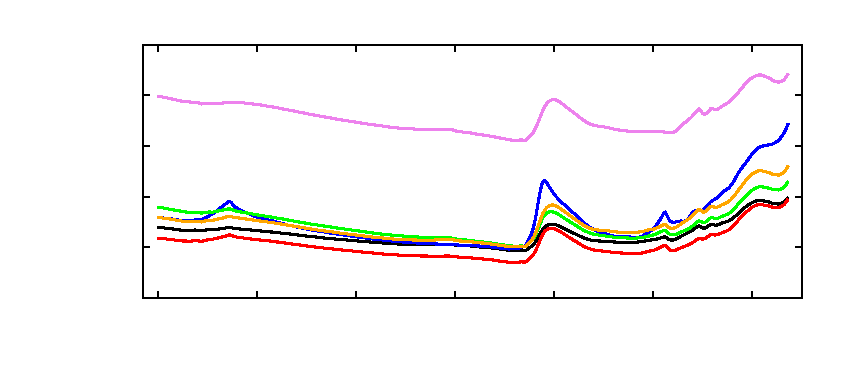
\includegraphics{gp/soil-spec-rnd}}%
    \gplfronttext
  \end{picture}%
\endgroup

			\caption{This figure shows near infrared soil spectra of six randomly chosen soil samples obtained from the used dataframe.}
			\label{fig:soil-spec-rnd}
		\end{figure*}

		The dataframe is made up of $533$ measured soil samples.
		For everyone of them the in section \ref{ssec:soil-parameters} discussed parameters $p_\m{SOC},p_\m{N},\m{pH}$ and the near infrared spectrum are given.
		The soil spectra consists of $319$ wavelengths ranging from $1400\unit{nm}$ to $2672\unit{nm}$ by a step of $4\unit{nm}$.
		The reflectance $\varrho(\lambda)$ of a sample at a given wavelength $\lambda$ is saved as
		\[
			-\lg \varrho(\lambda) = -\frac{\ln \varrho(\lambda)}{\ln 10}
		\]
		Figure \ref{fig:soil-spec-rnd} shows six randomly chosen soil spectra in a diagram.
	
	% subsection measured-data

	\subsection{Statistical Model}
	\label{ssec:statistical-model}
	
		Let $n\in\SN$ be the soil sample count and $k\in\SN$ with $k\leq n$ the number of measured wavelengths.
		$\varrho_i$ shall be defined as soil spectrum of the $i$th sample for every $i\in\SN,i\leq n$.
		$\lambda_j$ is the $j$th measured wavelength for every $j\in\SN,j\leq k$, also called predictor.
		Then according to section \ref{ssec:measured-data} the measured reflectance values are $x_{ij}$ with
		\[
			x_{ij} \define -\lg \varrho_i(\lambda_j)
		\]
		for every $i,j\in\SN,i\leq n,j\leq k$.
		Through the following matrix it is possible to get an easier notation.
		\[
			X \define (x_{ij}) \in \SR^{n\times k}
		\]
		Let $p^\m{(SOC)}_i, p^\m{(N)}_i, \m{pH}_i$ be the measured soil parameters of the $i$th sample for every $i\in\SN,i\leq n$, also known as observables.
		Then we define the $n$-dimensional vectors
		\begin{alignat*}{3}
			p^\m{(SOC)} &\define&&\ \curvb{p^\m{(SOC)}_i} \\
			p^\m{(N)} &\define&&\ \curvb{p^\m{(N)}_i} \\
			\m{pH} &\define&&\ \curvb{\m{pH}_i}
		\end{alignat*}

		The Beer-Lambert law allows us to make assumptions to the relations of soil spectra and soil parameters.
		In section \ref{ssec:nirs} we saw that the logarithmized reflectance can be written as a linear combination of molar concentrations.
		Hence, vice versa it makes sense to assume that an ASF can be represented by a linear combination of logarithmized reflectance values.

		Now let $P^\m{(SOC)},P^\m{(N)}$ be the appropriate random variables to the soil parameters $p^\m{(SOC)}$ and $p^{(N)}$.
		Then with the above assumption the expected values are given by
		\begin{alignat*}{3}
			\expect P^\m{(SOC)} &=&&\ X\beta^\m{(SOC)}_k + \beta^\m{(SOC)}_0 \definedby \mathbb{X}\beta^\m{(SOC)} \\
			\expect P^\m{(N)} &=&&\ X\beta^\m{(N)}_k + \beta^\m{(N)}_0 \definedby \mathbb{X}\beta^\m{(N)}
		\end{alignat*}
		When $\m{PH}$ is the corresponding random variable to $\m{pH}$ we have to perform a correction because $\m{pH}$ is a logarithmized molar concentration.
		It makes sense to model these with the subsequent expected value.
		\[
			\expect \m{PH} = \ln(X)\beta^\m{(pH)}_k + \beta^\m{(pH)}_0 \definedby \mathbb{X}_{\ln}\beta^\m{(pH)}
		\]

		In physics and chemistry it is a common and error-proven method to assume a normal distribution with a certain variance for measuring errors.
		So with the variances $(\sigma^2)^\m{(SOC)},(\sigma^2)^\m{(N)},(\sigma^2)^\m{(pH)}\in(0,\infty)$ our random variables become
		\begin{alignat*}{3}
			P^\m{(SOC)} &\sim&&\ \FN\curvb{\mathbb{X}\beta^\m{(SOC)}, (\sigma^2)^\m{(SOC)}\idmat_n} \\
			P^\m{(N)} &\sim&&\ \FN\curvb{\mathbb{X}\beta^\m{(N)}, (\sigma^2)^\m{(N)}\idmat_n} \\
			\m{PH} &\sim&&\ \FN\curvb{\mathbb{X}_{\ln}\beta^\m{(pH)}, (\sigma^2)^\m{(pH)}\idmat_n}
		\end{alignat*}
	
	% subsection statistical-model

	\subsection{MLR}
	\label{ssec:mlr}
	
		Multiple linear regression (MLR) or multivariate linear regression is a statistical method for estimating parameters that depend on linear independent variables.
		Let $\mathbb{X}\in\SR^{n\times(k+1)}, n,k\in\SN,k<n$ be the design matrix, $\sigma^2\in(0,\infty)$ and $Y$ be the vector of random variables with
		\[
			Y \sim \FN\curvb{\mathbb{X}\beta,\sigma^2\idmat_n}
		\]
		for a certain $\beta\in\SR^{k+1}$
		Then through the maximum-likelihood-method and a small correction we get two best unbiased estimators $\hat{\beta},\hat{\sigma^2}$ for $\beta$ and $\sigma^2$
		\begin{alignat*}{3}
			\hat{\beta}(Y) &=&&\ \inv{\curvb{\transp{\mathbb{X}}\mathbb{X}}}\transp{\mathbb{X}}Y \\
			\hat{\sigma^2}(Y) &=&&\ \frac{1}{n-(k+1)}\norm{Y - \mathbb{X}\hat{\beta}(Y)}^2
		\end{alignat*}
		Now let $y \define (y_i)\in\SR^n$ be a realization of $Y$.
		In this case we define
		\begin{alignat*}{3}
			\hat{y} &\define&&\ \mathbb{X}\hat{\beta}(y) = \mathbb{X}\inv{\curvb{\transp{\mathbb{X}}\mathbb{X}}}\transp{\mathbb{X}}y \\
			\hat{\sigma^2} &\define&&\ \hat{\sigma^2}(y)
		\end{alignat*}
		For more information please refer to [Quelle:Skript,wikipedia].
	
	% subsection mlr

	\subsection{Mallows' $\m{Cp}$}
	\label{ssec:mallows-cp}
	
		According to sections \ref{ssec:statistical-model} and \ref{ssec:mlr} at this time we are using $k+1 = 320$ predictors for our prediction model.
		Estimating Model Parameters with this large amount of predictors tends to overfit the measured data.
		% Quelle: Tutorial, Skript
		So it would be sensible to choose a \enquote{good} subset of predictors
		\[
			M\subset \set[i\in\SN_0,i\leq k]{\lambda_i}
		\]
		where $\lambda_0$ stands for the defined offset.
		Now through $M$ one can define a new design matrix $\mathbb{X}^{(M)}$.
		Applying MLR to this design matrix gives us new estimators
		\begin{alignat*}{3}
			\hat{\beta}^{(M)}(Y) &=&&\ \inv{\curvb{\transp{\mathbb{X}^{(M)}}\mathbb{X}^{(M)}}}\transp{\mathbb{X}^{(M)}}Y \\
			\hat{\sigma^2}^{(M)}(Y) &=&&\ \frac{1}{n-\#M}\norm{Y - \mathbb{X}^{(M)}\hat{\beta}^{(M)}(Y)}^2
		\end{alignat*}
		
		The term \enquote{good} refers to a criterion by which we can define the \enquote{goodness} of $M$.
		Here we will use Mallows' $\m{Cp}$.
		\[
			\m{Cp}^{(M)} \define \frac{1}{\hat{\sigma^2}}\sum_{i=1}^n\curvb{y_i-\hat{y}^{(M)}_i}^2 - n + 2\#M
		\]
		The minimization this value is equivalent to the minimization of the sum of predicted squared errors (SPSE).
	
	% subsection mallows-cp

	\subsection{Simulated Annealing}
	\label{ssec:simulated-annealing}
	
		The set of predictors contains $k=319$ free selectable elements (the constant shall remain).
		Therefore the power set $\s{P}$, the set of possible subsets $M$, contains of $2^{k}=2^{319}$ elements.
		If we want to find a subset $M$ so that for all $N\in\s{P}$ the inequation holds
		\[
			\m{Cp}^{(M)} \leq \m{Cp}^{(N)}
		\]
		we have to calculate $\m{Cp}^{(N)}$ for every $N\in\s{P}$.
		But this is a calculation beyond our current computing power.

		Simulated annealing (SA) is a probabilistic technique for approximating the global optimum of a given function.
		Specifically, it is a metaheuristic to approximate global optimization in a large search space.
		% Quelle: https://en.wikipedia.org/wiki/Simulated_annealing
		With this algorithm it is possible to find a good local minimum in a short time.
	
	% subsection simulated-annealing

% section fundamentals
	\section{Methodology}
\label{sec:methodology}
	
	\subsection{Measured Data}
	\label{ssec:measured-data}
	
		As a single spectrum contains overlapping information, it is necessary to determine both relevant wavelengths and the respective parameters to apply NIRS to practical problems.
		To select wavelengths and determine parameters we use an example data set, which contains $p^\m{(SOC)},p^\m{(N)},\m{pH}$ and wave reflectances of 319 wavelengths ranging from $1400 \unit{nm}$ to $2672 \unit{nm}$ by steps of $4 \unit{nm}$ for 533 samples \cite{don:a}.

		We define $\Lambda$ as the set of all measured wavelengths. The reflectance $\varrho(\lambda)$ of a sample at a wavelength $\lambda \in \Lambda$ is recorded as
		\[
			-\lg \varrho(\lambda) = -\frac{\ln \varrho(\lambda)}{\ln 10}
		\]
		Figure \ref{fig:soil-spec-rnd} shows six randomly chosen soil spectra in a diagram.
		\begin{figure*}
			\centering
			% GNUPLOT: LaTeX picture with Postscript
\begingroup
  \makeatletter
  \providecommand\color[2][]{%
    \GenericError{(gnuplot) \space\space\space\@spaces}{%
      Package color not loaded in conjunction with
      terminal option `colourtext'%
    }{See the gnuplot documentation for explanation.%
    }{Either use 'blacktext' in gnuplot or load the package
      color.sty in LaTeX.}%
    \renewcommand\color[2][]{}%
  }%
  \providecommand\includegraphics[2][]{%
    \GenericError{(gnuplot) \space\space\space\@spaces}{%
      Package graphicx or graphics not loaded%
    }{See the gnuplot documentation for explanation.%
    }{The gnuplot epslatex terminal needs graphicx.sty or graphics.sty.}%
    \renewcommand\includegraphics[2][]{}%
  }%
  \providecommand\rotatebox[2]{#2}%
  \@ifundefined{ifGPcolor}{%
    \newif\ifGPcolor
    \GPcolorfalse
  }{}%
  \@ifundefined{ifGPblacktext}{%
    \newif\ifGPblacktext
    \GPblacktexttrue
  }{}%
  % define a \g@addto@macro without @ in the name:
  \let\gplgaddtomacro\g@addto@macro
  % define empty templates for all commands taking text:
  \gdef\gplbacktext{}%
  \gdef\gplfronttext{}%
  \makeatother
  \ifGPblacktext
    % no textcolor at all
    \def\colorrgb#1{}%
    \def\colorgray#1{}%
  \else
    % gray or color?
    \ifGPcolor
      \def\colorrgb#1{\color[rgb]{#1}}%
      \def\colorgray#1{\color[gray]{#1}}%
      \expandafter\def\csname LTw\endcsname{\color{white}}%
      \expandafter\def\csname LTb\endcsname{\color{black}}%
      \expandafter\def\csname LTa\endcsname{\color{black}}%
      \expandafter\def\csname LT0\endcsname{\color[rgb]{1,0,0}}%
      \expandafter\def\csname LT1\endcsname{\color[rgb]{0,1,0}}%
      \expandafter\def\csname LT2\endcsname{\color[rgb]{0,0,1}}%
      \expandafter\def\csname LT3\endcsname{\color[rgb]{1,0,1}}%
      \expandafter\def\csname LT4\endcsname{\color[rgb]{0,1,1}}%
      \expandafter\def\csname LT5\endcsname{\color[rgb]{1,1,0}}%
      \expandafter\def\csname LT6\endcsname{\color[rgb]{0,0,0}}%
      \expandafter\def\csname LT7\endcsname{\color[rgb]{1,0.3,0}}%
      \expandafter\def\csname LT8\endcsname{\color[rgb]{0.5,0.5,0.5}}%
    \else
      % gray
      \def\colorrgb#1{\color{black}}%
      \def\colorgray#1{\color[gray]{#1}}%
      \expandafter\def\csname LTw\endcsname{\color{white}}%
      \expandafter\def\csname LTb\endcsname{\color{black}}%
      \expandafter\def\csname LTa\endcsname{\color{black}}%
      \expandafter\def\csname LT0\endcsname{\color{black}}%
      \expandafter\def\csname LT1\endcsname{\color{black}}%
      \expandafter\def\csname LT2\endcsname{\color{black}}%
      \expandafter\def\csname LT3\endcsname{\color{black}}%
      \expandafter\def\csname LT4\endcsname{\color{black}}%
      \expandafter\def\csname LT5\endcsname{\color{black}}%
      \expandafter\def\csname LT6\endcsname{\color{black}}%
      \expandafter\def\csname LT7\endcsname{\color{black}}%
      \expandafter\def\csname LT8\endcsname{\color{black}}%
    \fi
  \fi
  \setlength{\unitlength}{0.0500bp}%
  \begin{picture}(7936.00,3400.00)%
    \gplgaddtomacro\gplbacktext{%
      \csname LTb\endcsname%
      \put(1078,704){\makebox(0,0)[r]{\strut{} 0.3}}%
      \put(1078,1190){\makebox(0,0)[r]{\strut{} 0.35}}%
      \put(1078,1676){\makebox(0,0)[r]{\strut{} 0.4}}%
      \put(1078,2163){\makebox(0,0)[r]{\strut{} 0.45}}%
      \put(1078,2649){\makebox(0,0)[r]{\strut{} 0.5}}%
      \put(1078,3135){\makebox(0,0)[r]{\strut{} 0.55}}%
      \put(1353,484){\makebox(0,0){\strut{} 1400}}%
      \put(2304,484){\makebox(0,0){\strut{} 1600}}%
      \put(3256,484){\makebox(0,0){\strut{} 1800}}%
      \put(4208,484){\makebox(0,0){\strut{} 2000}}%
      \put(5160,484){\makebox(0,0){\strut{} 2200}}%
      \put(6111,484){\makebox(0,0){\strut{} 2400}}%
      \put(7063,484){\makebox(0,0){\strut{} 2600}}%
      \put(176,1919){\rotatebox{-270}{\makebox(0,0){\strut{}$-\lg \varrho(\lambda)$}}}%
      \put(4374,154){\makebox(0,0){\strut{}$\lambda \ [\m{nm}]$}}%
    }%
    \gplgaddtomacro\gplfronttext{%
    }%
    \gplbacktext
    \put(0,0){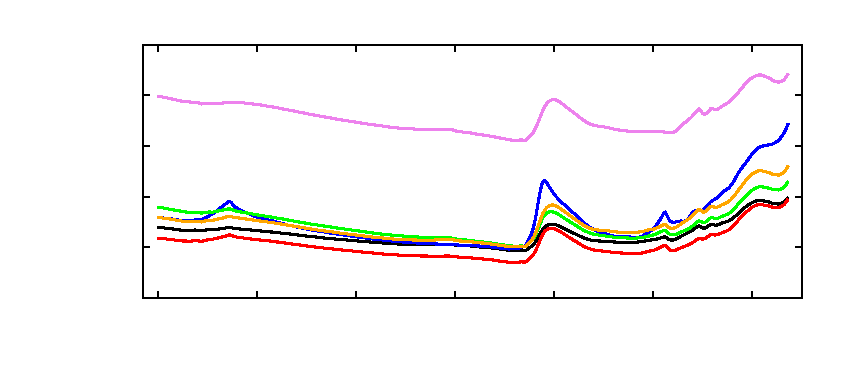
\includegraphics{gp/soil-spec-rnd}}%
    \gplfronttext
  \end{picture}%
\endgroup

			\caption{Six near infrared soil spectra of randomly chosen soil samples obtained from the data set, where $\lambda$ is the wavelength and $\rho(\lambda)$ the corresponding reflectance and each colour refers to one sample}
			\label{fig:soil-spec-rnd}
		\end{figure*}
		
	
	% subsection measured-data

	\subsection{Statistical Model}
	\label{ssec:statistical-model}
	
		Let $n\in\SN$ be the size of the data set and $k\in\SN$ with $k< n$ the number of measured wavelengths. We define
		$\varrho_i$ as the soil spectrum of the $i$th sample for every $i\in\SN,i\leq n$.
		$\lambda_j$ is the $j$th measured wavelength for every $j\in\SN,j\leq k$. We will alternatively refer to these as predictors.%note that we might have to introduce the term predictor at this point
		Then according to section \ref{ssec:measured-data} the measured reflectance values are $x_{ij}$ with
		\[
			x_{ij} \define -\lg \varrho_i(\lambda_j)
		\]
		for every $i,j\in\SN,i\leq n,j\leq k$.
		
	
		We define the measured ASF of $\m{SOC}$ of the $i$th sample for every $i\in\SN,i\leq n$ as $p^\m{(SOC)}_i$ to which we will also refer to as response variable.
		To simplify notation, we then define the $n$-dimensional vector
		\[
			p^\m{(SOC)} \define \curvb{p^\m{(SOC)}_i}
		\]

		The Beer-Lambert law allows us to make assumptions on the relations between soil spectra and the response variable \cite[247-8, 254]{agelet:10a}.
		We saw in section \ref{ssec:nirs} that the logarithmised reflectance can be written as a linear combination of molar concentrations.
		Hence, it seems plausible to assume that an ASF can be represented by a linear combination of logarithmised reflectance values.

		Now let $P^\m{(SOC)}$ be the appropriate random vector to $p^\m{(SOC)}$.
		Then under the above assumption the expected values are given for all $i \in \SN, i \leq n$ by
		\[
			\expect P_i^\m{(SOC)} \define \beta^\m{(SOC)}_0 + \sum_{j = 1}^k{x_{ij}\beta^\m{(SOC)}_j} 
		\]
		which simplifies with an $\mathbb{X} \in \SR^{n \times (k+1)}$, called design matrix, and a parameter vector $\beta^\m{(SOC)} \in \SR^{k+1}$ to
		\[
			\expect P^\m{(SOC)} = \mathbb{X}\beta^\m{(SOC)}
		\]
		
		To capture the stochastic part of $P^\m{(SOC)}$, we extend the model to
		\begin{alignat*}{3}
			&P^\m{(SOC)} = \mathbb{X}\beta^\m{(SOC)} + \varepsilon^\m{(SOC)} \\
			&\expect \varepsilon^\m{(SOC)} = 0, \qquad \cov \varepsilon^\m{(SOC)} = (\sigma^2)^\m{(SOC)} \idmat
		\end{alignat*}
		where $(\sigma^2)^\m{(SOC)} \in (0,\infty)$. Following common practice in physics and chemistry, we further assume that 
		\[
			\varepsilon^\m{(SOC)} \sim \FN \curvb{0,(\sigma^2)^\m{(SOC)}\idmat}
		\]
		This results in the complete model
		\[
			P^\m{(SOC)} \sim \FN \curvb{\mathbb{X}\beta^\m{(SOC)},(\sigma^2)^\m{(SOC)} \idmat}
		\]
		The model for the second response variable $P^\m{(N)}$ is constructed in analogy.
		
		The case for the $\m{pH}$ is slightly different, though. 
		When modelling the corresponding random variable we have to adjust the model as the $\m{pH}$ is a logarithmised molar concentration.
		We therefore have to include this into the expected value of the corresponding random variables
		
		\[
			\expect \m{\overline{pH}}_i \define \beta^\m{\m{(pH)}}_0 + \sum_{j = 1}^k{\ln (x_{ij}) \beta^\m{(pH)}_j} 
		\]
		and denote the corresponding matrix by $\mathbb{X}_{\ln}$.

	
	% subsection statistical-model

	\subsection{Multivariate Linear Regression}
	\label{ssec:mlr}
	
		Multivariate linear regression (MLR) is a statistical method for finding parameters of linear relations between a response variable and a set of predictors.
		These can be reused to predict new responses \cite{draper:98a, pardoe:12a, schumacher:16a}
		Let $\mathbb{X}\in\SR^{n\times(k+1)}, n,k\in\SN,k<n$ be the design matrix with $\rank{\mathbb{X}} = k+1$, $\sigma^2\in(0,\infty)$ and $Y$ be the random vector of a response variable with
		\[
			Y \sim \FN\curvb{\mathbb{X}\beta,\sigma^2\idmat_n}
		\]
		for a certain $\beta\in\SR^{k+1}$
		Then through the maximum-likelihood-method and a correction we get two best unbiased estimators $\hat{\beta},\hat{\sigma}^2$ for $\beta$ and $\sigma^2$
		\begin{alignat*}{3}
			\hat{\beta}(Y) &=&&\ \inv{\curvb{\transp{\mathbb{X}}\mathbb{X}}}\transp{\mathbb{X}}Y \\
			\hat{\sigma}^2(Y) &=&&\ \frac{1}{n-(k+1)}\norm{Y - \mathbb{X}\hat{\beta}(Y)}^2
		\end{alignat*}
		Now let $y \define (y_i)\in\SR^n$ be a realization of $Y$.
		Then we define
		\begin{alignat*}{3}
			\hat{y} &\define&&\ \mathbb{X}\hat{\beta}(y) = \mathbb{X}\inv{\curvb{\transp{\mathbb{X}}\mathbb{X}}}\transp{\mathbb{X}}y \\
			\widehat{{\sigma}^2} &\define&&\ \hat{\sigma}^2(y)
		\end{alignat*}

	% subsection mlr

	\subsection{Mallows' $\m{C_p}$}
	\label{ssec:mallows-C_p}
	
		At this point, the model is specified using $k+1 = 320$ predictors for each response variable, using the whole measured spectra for each soil sample.
		This set of predictors is comparatively large, $n-k < k$.
		Further, the reflectances of neighbouring lightwaves are correlated \cite[252]{agelet:10a}.
		In these circumstances, we might overfit the data, i.e. the variance of our estimated parameters $\hat{\beta}_i(Y)$ might be too large, compromising their usability for future measurements.
		To address this problem, it is sensible to limit each actual model to a \enquote{good} subset of the predictors. Hence, our task becomes to select the best or at least a \enquote{sufficiently} good model $M$ defined by
		\[
			M\subset \Lambda \cup \set{\lambda_0} \definedby \overline{\Lambda}
		\]
		where $\lambda_0$ stands for the intercept.
		We denote the design matrix for each $M$ by $\mathbb{X}^{(M)}$.
		Applying MLR to the new design matrix yields the new estimators
		\begin{alignat*}{3}
			\hat{\beta}^{(M)}(Y) &=&&\ \inv{\curvb{\transp{\mathbb{X}^{(M)}}\mathbb{X}^{(M)}}}\transp{\mathbb{X}^{(M)}}Y \\
			\curvb{\hat{\sigma}^2}^{(M)}(Y) &=&&\ \frac{1}{n-\m{p}}\norm{Y - \mathbb{X}^{(M)}\hat{\beta}^{(M)}(Y)}^2_2,
		\end{alignat*}
		where $\m{p} \in \set{1,\ldots,k+1}$ corresponds to the number of predictors included in $M$.
		
		The sum of predicted squared errors ($\m{SPSE}$) is a theoretical criterion to compare the merits of different models.
		The $\m{SPSE}$ measures how well a model does in predicting new responses from new data:
		\[
			\m{SPSE}^{(M)} \define \sum_{i = 1}^n \expect \curvb{Y_{n+i} - \hat{Y}_i^{(M)}}^2
		\]
		which simplifies to \cite[29-30]{schumacher:16a}
		\[
			\m{SPSE}^{(M)} = n\sigma^2 + \m{p}\sigma^2 + \curvb{\m{bias}^2}^{(M)}
		\]
		where $\m{bias}$ describes the divergence of the true expectation from the estimated expection.
		As it decreases in the number of included parameters, we assume it to be close enough to zero and neglect it from our further considerations.
		
		Unfortunately, the true $\sigma^2$ is unobservable so that it has to be estimated by
		\[
			\widehat{\m{SPSE}}^{(M)}(Y) \define \norm{Y - \mathbb{X}^{(M)}\hat{\beta}^{(M)}(Y)}^2_2 + 2\m{p}\hat{\sigma}^2(Y)
		\]
		
		Instead of using the $\widehat{\m{SPSE}}^{(M)}$ directly, we will use Mallow's $C_\m{p}$ instead, given by
		\[
			\m{C_p}^{(M)} \define \frac{1}{\widehat{{\sigma}^2}}\sum_{i=1}^n\curvb{y_i-\hat{y}^{(M)}_i}^2 - n + 2\m{p}
		\]
		Minimising this value is equivalent to the minimisation of the $\widehat{\m{SPSE}}^{(M)}$.
		% The proof is trivial, just biject it to a conext-free residue class, whose elements are open manifolds. %citation
	
	% subsection mallows-C_p

	\subsection{Simulated Annealing}
	\label{ssec:model-selec}
	
		We can now formulate the following minimisation problem.
		Let
		\[
			\s{H} \define \set[A\in\setpow(\Lambda)]{A \cup \set{\lambda_0}} \subset \setpow\curvb{\overline{\Lambda}}
		\]
		Then the model we want to select is a solution to
%		\[
%			\curvb{\Omega} \qquad \minimize_{M\in\s{H}} \qquad C_\m{p}^{(M)}
%		\]
		\[
			\Omega \define \minimize \; \set[M\in\s{H}]{C_\m{p}^{(M)}}
		\]
		This problem is a discrete optimisation problem, which is in general np-hard \cite[245-50]{schrijver:98a}.
		Unfortunately, $\abs{\s{H}} = 2^{319}$, which is too large for a complete search.
		Therefore, we need a heuristic search algorithm that does not depend on further information of the cost function.

		Simulated annealing (SANN) is a heuristic algorithm that approximates global optima of a given function \cite[549-54]{press:07a}.
		Note that the SANN returns only a probabilistically good approximation $\s{M}\in\s{H}$ to a true solution to $\Omega$.
		Lacking similarly reliable and computationally feasible alternatives we use the solution returned by SANN instead.

		The algorithm is applicable to arbitrary sets, in our case $\s{H}$.
		It simulates the slow cooling of a thermodynamic system.
		Let $x_0\in\s{H}$ be the initial set of predictors, $T_0\in(0,\infty)$ be the initial temperature of the system and $i_\m{max}\in\SN$ be the maximal number of time steps.
		Then the algorithm requires the following functions:
		\begin{itemize}
			\item $\func{\m{cost}}{\s{H}}{\SR}$ \\
				Calculates the cost of a given predictor set.
			\item $\func{\m{temp}}{\SR\times\SN^2}{(0,\infty)}$\\
				Calculates the temperature according to the given initial temperature and time steps.
				It is a monotonically decreasing function in the second parameter.
			\item $\func{\m{nbr}}{\s{H}}{\s{H}}$ \\
				Generates a random neighbour of a given predictor set.
			\item $\func{\m{prob}}{\SR^2\times(0,\infty)}{[0,1]}$ \\
				Calculates the probability of changing the current set or state to the neighbour.
			\item $\m{rnd}(0,1)$ \\
				Returns a random number in the interval $[0,1]$.
		\end{itemize}
		The listing shows one variant of the pseudocode of the SANN algorithm. 

		\medskip
		\begin{tcolorbox}[colframe=black,colbacktitle=white,coltitle=black, attach boxed title to top center={yshift=-2mm},enhanced, titlerule=0.1pt, boxrule=0.5pt, arc=5pt,title=Listing:\quad SANN algorithm]
			\begin{tabbing}
	\qquad\=\qquad\=\qquad\=\qquad\=\kill
	$c_0 = \m{cost}(x_0)$\\
	\\
	\textbf{for} ($i=1$, $i\leq i_\m{max}$) \{\\
		\>$T = \m{temp}(T_0,i,i_\m{max})$\\
		\\
		\>$x_1 = \m{nbr}(x_0)$\\
		\>$c_1 = \m{cost}(x_1)$\\
		\\
		\>\textbf{if} $(\m{prob}(c_0, c_1, T) \geq \m{rnd}(0,1))$ \{\\
			\>\>$x_0 = x_1$\\
			\>\>$c_0 = c_1$\\
		\>\}\\
	\}
\end{tabbing}
		\end{tcolorbox}
		\medskip

	% subsection simulated-annealing
		
	\subsection{Model Validation}
	\label{ssec:model-validation}
	
		To examine the models selected by SANN, we recur to the often used $R^2$ measure \cite[33-4]{draper:98a}.
		For $M\in\s{H}$ it is given by
		\[
			\curvb{R^2}^{(M)} \define \frac {\sum_{i=1}^n \curvb{\hat{y}^{(M)}_i - \overline{y}}^2}{\sum_{i=1}^n \curvb{y_i - \overline{y}}^2} \in [0,1]
		\]
		where $\overline{y}$ is the arithmetic mean of $y_i$ for $i=1,\ldots,n$ and describes how much of the total variation of $y$ is explained by the model $M$.
		$\curvb{R^2}^{(M)} = 0$ is equivalent to no, $\curvb{R^2}^{(M)} = 1$ to full agreement of the model with the observations.
		
		We shall note though, that the measure is increasing with $\abs{M}$.
		In contrast the actual upper bound of $R^2$ is lowered by the presence of measurement errors.
		We will therefore consult the correlation diagrams for each response variable observation vector and its respective prediction vector to complement our judgement based on the $R^2$ measure.

	% subsection model-validation
	
	\subsection{Simulation}
	\label{ssec:simulation}
	
		As the true $\m{SPSE}$ is unobservable, we need to assess how well our procedure minimises the true $\m{SPSE}$ in general.
		For limitations of available data we have to resort to so called pseudo-observations of a response variable, which we collect in a random vector as follows
		\[
			\widetilde{Y} \define \hat{y}^{(\s{M})} + \varepsilon,\qquad \varepsilon \sim  \FN \curvb{0,\sigma^2\idmat_n}
		\]
		where we assign
		\[
			\sigma^2 \define \curvb{\widehat{\sigma^2}}^{(\s{M})}
		\]
		Having fixed the parameters for the random vector $\widetilde{Y}$ we can now calculate the true $\m{SPSE}$ from them by
		\[
			\m{SPSE}^{(\s{M})} = \curvb{ n + \abs{\s{M}} } \sigma^2
		\]
		
		We can now simulate a new application of our model selection algorithm for
		\[
			\widetilde{Y} \sim \FN\curvb{\mathbb{X}\widetilde{\beta},\sigma^2\idmat_n}
		\]
		treating $\sigma^2$ as unknown.
		The algorithm returns a model $\widetilde{\s{M}}$. We can now calculate $\widehat{\m{SPSE}}^{(\widetilde{\s{M}})}$ and compare it to the true $\m{SPSE}$.
		Due to the heuristic nature of the selection algorithm, we might end up with an exceptionally bad value.
		To address this, we repeat this process $r$ times \cite{schumacher:16b}.
		
		In addition to parameters of the random vector $\widetilde{Y}$, $\widehat{\m{SPSE}}^{(\widetilde{\s{M}})}$ depends on the hyperparameters, resolution $k = \abs{\Lambda}$ and the number of observations, $n$, as well.
		To gauge influences of the resolution on the model selection, we augment the procedure above to include the sets
		\[
			\Lambda^{(m)} \define \set[i\in\SN, m \cdot i \leq k]{\lambda_{m\cdot i} \in \Lambda}
		\]
		where $m \in \set{1, 2, 3, 4}$ and $\Lambda^{(m)}$ takes replace of $\Lambda$ in \ref{ssec:mallows-C_p} and \ref{ssec:model-selec}.
		
		To assess the influence of the number of available measurements, we choose randomly selected subsets of the existing measurements of sizes $n \in \set{100, 200, 300, 500, 533}$ and augment the simulation accordingly.
		In this way, we can compare the $\widehat{\m{SPSE}}^{(\widetilde{\s{M}})}$ with the \enquote{true} model's $\m{SPSE}$ in 19 situations and on the same $r$ pseudo-observations for each.
		
	% subsection simulation
% section methodology
	\section{Implementation}
\label{sec:implementation}
	
	\subsection{Choosing a Neighbour}
	\label{ssec:choosing-a-neighbour}
		
		We stated in section \ref{ssec:model-selec} that we want to select a \enquote{good} model for the prediction.
		To this goal, we have to define the functions and parameters of the algorithm.
		The most important one is the $\m{nbr}$ function whose purpose is to choose a neighbour efficiently since the final solution depends on a sequence of neighbours.
		In most cases it is best to select a neighbour not too far away from the given subset. %citation!
		% Quelle: https://en.wikipedia.org/wiki/Simulated_annealing

		Our $\m{nbr}$ function generates a random natural number $r\in\set{1,\ldots,k}$ that represents the index of a measured wavelength.
		If this predictor is already in our current subset then we remove it.
		If not, we include it to the new subset.
		That way, new neighbours are not too far away from the current parameter vector.
		The pseudocode is shown in the following listing.
		\medskip
		\begin{tcolorbox}[colframe=black,colbacktitle=white,coltitle=black, attach boxed title to top center={yshift=-2mm},enhanced, titlerule=0.1pt, boxrule=0.5pt, arc=5pt,title=Listing:\quad $\m{nbr}$ function]
			\begin{tabbing}
	\qquad\=\qquad\=\qquad\=\qquad\=\kill
	\textbf{function} $\m{nbr}(M)$\{\\
		\>$r = \m{rnd}\set{2,\ldots,k+1}$\\
		\\
		\>\textbf{if} ($\lambda_r\in M$)\{\\
			\>\>$\tilde{M}=M\setminus\set{\lambda_r}$\\
		\>\}\textbf{else}\{\\
			\>\>$\tilde{M}=M\cup\set{\lambda_r}$\\
		\>\}\\
		\\
		\>\textbf{return} $\tilde{M}$\\
	\}
\end{tabbing}
		\end{tcolorbox}
		\medskip
	% subsection choosing-a-neighbour
		
	\subsection{Additional Functions}
	\label{ssec:add-func}
	
		All other functions were defined following a standard scheme.
		It follows from \ref{ssec:mallows-C_p} that
		\[
			\m{cost}(M)\define \m{C_p}^{(M)}
		\]
		In most applications $\m{prob}$ is defined in analogy to the transition of a physical system.
		%here we need maybe some elaboration
		% Quelle: https://en.wikipedia.org/wiki/Simulated_annealing
		\[
			\m{prob}(c_0,c_1,T) \define \exp\curvb{\frac{c_0 - c_1}{T}}
		\]
		Details of $\m{temp}$ are not really important as long as it monotonically decreases in the second parameter.
		So let $\alpha\in(0,1)$.
		\[
			\m{temp}(T_0,i,i_\m{max})\define T_0\alpha^i
		\]
	%subsection Additional Functions
	
	\subsection{Preprocessing}
	\label{ssec:preprocessing}
	
		 Implementing the algorithm described in \ref{ssec:model-selec} takes a sizeable toll on computing power.
		 The most expensive calculations are performed in the computation of the residual sum of squares
		 \[
		 	\norm{y - \mathbb{X}^{(M)}\hat{\beta}^{(M)}(y)}^2_2
		 \] 
		 which requires the computation of
		 \[
		 	\hat{\beta}^{(M)}(y) = \inv{\curvb{\transp{\mathbb{X}^{(M)}}\mathbb{X}^{(M)}}}\transp{\mathbb{X}^{(M)}}y
		\]
		
		 Instead of solving this, it is more efficient to solve
		 \[
		 	\transp{\mathbb{X}^{(M)}}\mathbb{X}^{(M)}\hat{\beta}(y) = \transp{\mathbb{X}^{(M)}}y
		\]
		which can be done through QR-decomposition or an adequate alternative.
		
		The design matrices $\mathbb{X}^{(M)}$ are full rank by construction.
		It follows then from the definition of $M$ that we can define an injective, monotone increasing function
		\[
			\delta_M : \set{0,\ldots, \abs{M}-1} \rightarrow \set{0,\ldots, k}
		\]
		that maps the indices of the design matrix $\mathbb{X}^{(M)}$ to the indices of the full design matrix $\mathbb{X}$.
		We then only have to precompute $\transp{\mathbb{X}}\mathbb{X}$ and $\transp{\mathbb{X}}y$ and construct $\transp{\mathbb{X}^{(M)}}\mathbb{X}^{(M)}$ and $\transp{\mathbb{X}^{(M)}}y$ by 
		\begin{alignat*}{3}
		 	\transp{\mathbb{X}^{(M)}}\mathbb{X}^{(M)} &=&&\  \curvb{\angleb{x_{\delta(i)}, x_{\delta(j)}}} \\
			\transp{\mathbb{X}^{(M)}}y &=&&\ \curvb{\curvb{\transp{\mathbb{X}}y}_{\delta(i)}}
		\end{alignat*}
		for all $i,j\in M$ where $x_{\delta(i)}$ is the $\delta(i)$th column vector of $\mathbb{X}$.
		 
		$\curvb{\hat\sigma^2}^{(\overline{\Lambda})}$ is a constant, we can precompute the estimated variance of the complete model and its inverse as well.
		For each of the simulation sets that depend on $m$, this process has to be repeated though.

	% subsection Preprocessing
	
		
% section implementation
			\begin{figure*}
			\center
			% \subcaphangtrue
			\begin{subfigure}[t]{0.33\textwidth}
				\centerline{
					% GNUPLOT: LaTeX picture with Postscript
\begingroup
  \makeatletter
  \providecommand\color[2][]{%
    \GenericError{(gnuplot) \space\space\space\@spaces}{%
      Package color not loaded in conjunction with
      terminal option `colourtext'%
    }{See the gnuplot documentation for explanation.%
    }{Either use 'blacktext' in gnuplot or load the package
      color.sty in LaTeX.}%
    \renewcommand\color[2][]{}%
  }%
  \providecommand\includegraphics[2][]{%
    \GenericError{(gnuplot) \space\space\space\@spaces}{%
      Package graphicx or graphics not loaded%
    }{See the gnuplot documentation for explanation.%
    }{The gnuplot epslatex terminal needs graphicx.sty or graphics.sty.}%
    \renewcommand\includegraphics[2][]{}%
  }%
  \providecommand\rotatebox[2]{#2}%
  \@ifundefined{ifGPcolor}{%
    \newif\ifGPcolor
    \GPcolorfalse
  }{}%
  \@ifundefined{ifGPblacktext}{%
    \newif\ifGPblacktext
    \GPblacktexttrue
  }{}%
  % define a \g@addto@macro without @ in the name:
  \let\gplgaddtomacro\g@addto@macro
  % define empty templates for all commands taking text:
  \gdef\gplbacktext{}%
  \gdef\gplfronttext{}%
  \makeatother
  \ifGPblacktext
    % no textcolor at all
    \def\colorrgb#1{}%
    \def\colorgray#1{}%
  \else
    % gray or color?
    \ifGPcolor
      \def\colorrgb#1{\color[rgb]{#1}}%
      \def\colorgray#1{\color[gray]{#1}}%
      \expandafter\def\csname LTw\endcsname{\color{white}}%
      \expandafter\def\csname LTb\endcsname{\color{black}}%
      \expandafter\def\csname LTa\endcsname{\color{black}}%
      \expandafter\def\csname LT0\endcsname{\color[rgb]{1,0,0}}%
      \expandafter\def\csname LT1\endcsname{\color[rgb]{0,1,0}}%
      \expandafter\def\csname LT2\endcsname{\color[rgb]{0,0,1}}%
      \expandafter\def\csname LT3\endcsname{\color[rgb]{1,0,1}}%
      \expandafter\def\csname LT4\endcsname{\color[rgb]{0,1,1}}%
      \expandafter\def\csname LT5\endcsname{\color[rgb]{1,1,0}}%
      \expandafter\def\csname LT6\endcsname{\color[rgb]{0,0,0}}%
      \expandafter\def\csname LT7\endcsname{\color[rgb]{1,0.3,0}}%
      \expandafter\def\csname LT8\endcsname{\color[rgb]{0.5,0.5,0.5}}%
    \else
      % gray
      \def\colorrgb#1{\color{black}}%
      \def\colorgray#1{\color[gray]{#1}}%
      \expandafter\def\csname LTw\endcsname{\color{white}}%
      \expandafter\def\csname LTb\endcsname{\color{black}}%
      \expandafter\def\csname LTa\endcsname{\color{black}}%
      \expandafter\def\csname LT0\endcsname{\color{black}}%
      \expandafter\def\csname LT1\endcsname{\color{black}}%
      \expandafter\def\csname LT2\endcsname{\color{black}}%
      \expandafter\def\csname LT3\endcsname{\color{black}}%
      \expandafter\def\csname LT4\endcsname{\color{black}}%
      \expandafter\def\csname LT5\endcsname{\color{black}}%
      \expandafter\def\csname LT6\endcsname{\color{black}}%
      \expandafter\def\csname LT7\endcsname{\color{black}}%
      \expandafter\def\csname LT8\endcsname{\color{black}}%
    \fi
  \fi
  \setlength{\unitlength}{0.0500bp}%
  \begin{picture}(3118.00,2834.00)%
    \gplgaddtomacro\gplbacktext{%
      \csname LTb\endcsname%
      \put(594,688){\makebox(0,0)[r]{\strut{} 0}}%
      \csname LTb\endcsname%
      \put(594,1051){\makebox(0,0)[r]{\strut{} 2}}%
      \csname LTb\endcsname%
      \put(594,1414){\makebox(0,0)[r]{\strut{} 4}}%
      \csname LTb\endcsname%
      \put(594,1777){\makebox(0,0)[r]{\strut{} 6}}%
      \csname LTb\endcsname%
      \put(594,2139){\makebox(0,0)[r]{\strut{} 8}}%
      \csname LTb\endcsname%
      \put(594,2502){\makebox(0,0)[r]{\strut{} 10}}%
      \csname LTb\endcsname%
      \put(907,287){\makebox(0,0){\strut{} 0}}%
      \csname LTb\endcsname%
      \put(1270,287){\makebox(0,0){\strut{} 2}}%
      \csname LTb\endcsname%
      \put(1633,287){\makebox(0,0){\strut{} 4}}%
      \csname LTb\endcsname%
      \put(1996,287){\makebox(0,0){\strut{} 6}}%
      \csname LTb\endcsname%
      \put(2358,287){\makebox(0,0){\strut{} 8}}%
      \csname LTb\endcsname%
      \put(2721,287){\makebox(0,0){\strut{} 10}}%
    }%
    \gplgaddtomacro\gplfronttext{%
      \csname LTb\endcsname%
      \put(1089,2139){\makebox(0,0)[l]{\strut{}SOC}}%
    }%
    \gplbacktext
    \put(0,0){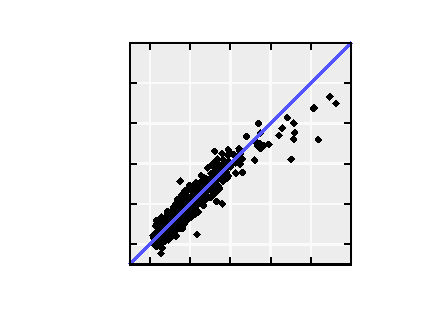
\includegraphics{gp/ms-sa-soc-corr}}%
    \gplfronttext
  \end{picture}%
\endgroup

				}
				\caption{\parbox[t]{0.45\textwidth}{
					$\hat{p}^{(\m{SOC})} \sim p^{(\m{SOC})}$ \smallskip \\
					$(R^2)^{(\m{SOC})} = 0.871$
					}}
			\end{subfigure}
			\begin{subfigure}[t]{0.33\textwidth}
				\centerline{
					% GNUPLOT: LaTeX picture with Postscript
\begingroup
  \makeatletter
  \providecommand\color[2][]{%
    \GenericError{(gnuplot) \space\space\space\@spaces}{%
      Package color not loaded in conjunction with
      terminal option `colourtext'%
    }{See the gnuplot documentation for explanation.%
    }{Either use 'blacktext' in gnuplot or load the package
      color.sty in LaTeX.}%
    \renewcommand\color[2][]{}%
  }%
  \providecommand\includegraphics[2][]{%
    \GenericError{(gnuplot) \space\space\space\@spaces}{%
      Package graphicx or graphics not loaded%
    }{See the gnuplot documentation for explanation.%
    }{The gnuplot epslatex terminal needs graphicx.sty or graphics.sty.}%
    \renewcommand\includegraphics[2][]{}%
  }%
  \providecommand\rotatebox[2]{#2}%
  \@ifundefined{ifGPcolor}{%
    \newif\ifGPcolor
    \GPcolorfalse
  }{}%
  \@ifundefined{ifGPblacktext}{%
    \newif\ifGPblacktext
    \GPblacktexttrue
  }{}%
  % define a \g@addto@macro without @ in the name:
  \let\gplgaddtomacro\g@addto@macro
  % define empty templates for all commands taking text:
  \gdef\gplbacktext{}%
  \gdef\gplfronttext{}%
  \makeatother
  \ifGPblacktext
    % no textcolor at all
    \def\colorrgb#1{}%
    \def\colorgray#1{}%
  \else
    % gray or color?
    \ifGPcolor
      \def\colorrgb#1{\color[rgb]{#1}}%
      \def\colorgray#1{\color[gray]{#1}}%
      \expandafter\def\csname LTw\endcsname{\color{white}}%
      \expandafter\def\csname LTb\endcsname{\color{black}}%
      \expandafter\def\csname LTa\endcsname{\color{black}}%
      \expandafter\def\csname LT0\endcsname{\color[rgb]{1,0,0}}%
      \expandafter\def\csname LT1\endcsname{\color[rgb]{0,1,0}}%
      \expandafter\def\csname LT2\endcsname{\color[rgb]{0,0,1}}%
      \expandafter\def\csname LT3\endcsname{\color[rgb]{1,0,1}}%
      \expandafter\def\csname LT4\endcsname{\color[rgb]{0,1,1}}%
      \expandafter\def\csname LT5\endcsname{\color[rgb]{1,1,0}}%
      \expandafter\def\csname LT6\endcsname{\color[rgb]{0,0,0}}%
      \expandafter\def\csname LT7\endcsname{\color[rgb]{1,0.3,0}}%
      \expandafter\def\csname LT8\endcsname{\color[rgb]{0.5,0.5,0.5}}%
    \else
      % gray
      \def\colorrgb#1{\color{black}}%
      \def\colorgray#1{\color[gray]{#1}}%
      \expandafter\def\csname LTw\endcsname{\color{white}}%
      \expandafter\def\csname LTb\endcsname{\color{black}}%
      \expandafter\def\csname LTa\endcsname{\color{black}}%
      \expandafter\def\csname LT0\endcsname{\color{black}}%
      \expandafter\def\csname LT1\endcsname{\color{black}}%
      \expandafter\def\csname LT2\endcsname{\color{black}}%
      \expandafter\def\csname LT3\endcsname{\color{black}}%
      \expandafter\def\csname LT4\endcsname{\color{black}}%
      \expandafter\def\csname LT5\endcsname{\color{black}}%
      \expandafter\def\csname LT6\endcsname{\color{black}}%
      \expandafter\def\csname LT7\endcsname{\color{black}}%
      \expandafter\def\csname LT8\endcsname{\color{black}}%
    \fi
  \fi
  \setlength{\unitlength}{0.0500bp}%
  \begin{picture}(3968.00,2834.00)%
    \gplgaddtomacro\gplbacktext{%
      \csname LTb\endcsname%
      \put(1018,677){\makebox(0,0)[r]{\strut{} 0}}%
      \csname LTb\endcsname%
      \put(1018,1150){\makebox(0,0)[r]{\strut{} 0.2}}%
      \csname LTb\endcsname%
      \put(1018,1623){\makebox(0,0)[r]{\strut{} 0.4}}%
      \csname LTb\endcsname%
      \put(1018,2096){\makebox(0,0)[r]{\strut{} 0.6}}%
      \csname LTb\endcsname%
      \put(1018,2569){\makebox(0,0)[r]{\strut{} 0.8}}%
      \csname LTb\endcsname%
      \put(1387,220){\makebox(0,0){\strut{} 0}}%
      \csname LTb\endcsname%
      \put(1860,220){\makebox(0,0){\strut{} 0.2}}%
      \csname LTb\endcsname%
      \put(2333,220){\makebox(0,0){\strut{} 0.4}}%
      \csname LTb\endcsname%
      \put(2806,220){\makebox(0,0){\strut{} 0.6}}%
      \csname LTb\endcsname%
      \put(3279,220){\makebox(0,0){\strut{} 0.8}}%
    }%
    \gplgaddtomacro\gplfronttext{%
      \csname LTb\endcsname%
      \put(1469,2250){\makebox(0,0)[l]{\strut{}$P^\m{(N)}$}}%
    }%
    \gplbacktext
    \put(0,0){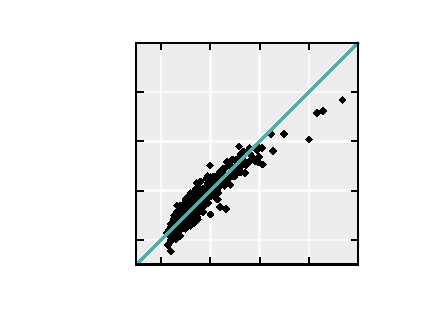
\includegraphics{gp/ms-sa-n-corr}}%
    \gplfronttext
  \end{picture}%
\endgroup

				}
				\caption{\parbox[t]{0.4\textwidth}{
					$\hat{p}^{(\m{N})} \sim p^{(\m{N})}$ \smallskip \\
					$(R^2)^{(\m{N})} = 0.861$
					}}
			\end{subfigure}
			\begin{subfigure}[t]{0.33\textwidth}
				\centerline{
					% GNUPLOT: LaTeX picture with Postscript
\begingroup
  \makeatletter
  \providecommand\color[2][]{%
    \GenericError{(gnuplot) \space\space\space\@spaces}{%
      Package color not loaded in conjunction with
      terminal option `colourtext'%
    }{See the gnuplot documentation for explanation.%
    }{Either use 'blacktext' in gnuplot or load the package
      color.sty in LaTeX.}%
    \renewcommand\color[2][]{}%
  }%
  \providecommand\includegraphics[2][]{%
    \GenericError{(gnuplot) \space\space\space\@spaces}{%
      Package graphicx or graphics not loaded%
    }{See the gnuplot documentation for explanation.%
    }{The gnuplot epslatex terminal needs graphicx.sty or graphics.sty.}%
    \renewcommand\includegraphics[2][]{}%
  }%
  \providecommand\rotatebox[2]{#2}%
  \@ifundefined{ifGPcolor}{%
    \newif\ifGPcolor
    \GPcolorfalse
  }{}%
  \@ifundefined{ifGPblacktext}{%
    \newif\ifGPblacktext
    \GPblacktexttrue
  }{}%
  % define a \g@addto@macro without @ in the name:
  \let\gplgaddtomacro\g@addto@macro
  % define empty templates for all commands taking text:
  \gdef\gplbacktext{}%
  \gdef\gplfronttext{}%
  \makeatother
  \ifGPblacktext
    % no textcolor at all
    \def\colorrgb#1{}%
    \def\colorgray#1{}%
  \else
    % gray or color?
    \ifGPcolor
      \def\colorrgb#1{\color[rgb]{#1}}%
      \def\colorgray#1{\color[gray]{#1}}%
      \expandafter\def\csname LTw\endcsname{\color{white}}%
      \expandafter\def\csname LTb\endcsname{\color{black}}%
      \expandafter\def\csname LTa\endcsname{\color{black}}%
      \expandafter\def\csname LT0\endcsname{\color[rgb]{1,0,0}}%
      \expandafter\def\csname LT1\endcsname{\color[rgb]{0,1,0}}%
      \expandafter\def\csname LT2\endcsname{\color[rgb]{0,0,1}}%
      \expandafter\def\csname LT3\endcsname{\color[rgb]{1,0,1}}%
      \expandafter\def\csname LT4\endcsname{\color[rgb]{0,1,1}}%
      \expandafter\def\csname LT5\endcsname{\color[rgb]{1,1,0}}%
      \expandafter\def\csname LT6\endcsname{\color[rgb]{0,0,0}}%
      \expandafter\def\csname LT7\endcsname{\color[rgb]{1,0.3,0}}%
      \expandafter\def\csname LT8\endcsname{\color[rgb]{0.5,0.5,0.5}}%
    \else
      % gray
      \def\colorrgb#1{\color{black}}%
      \def\colorgray#1{\color[gray]{#1}}%
      \expandafter\def\csname LTw\endcsname{\color{white}}%
      \expandafter\def\csname LTb\endcsname{\color{black}}%
      \expandafter\def\csname LTa\endcsname{\color{black}}%
      \expandafter\def\csname LT0\endcsname{\color{black}}%
      \expandafter\def\csname LT1\endcsname{\color{black}}%
      \expandafter\def\csname LT2\endcsname{\color{black}}%
      \expandafter\def\csname LT3\endcsname{\color{black}}%
      \expandafter\def\csname LT4\endcsname{\color{black}}%
      \expandafter\def\csname LT5\endcsname{\color{black}}%
      \expandafter\def\csname LT6\endcsname{\color{black}}%
      \expandafter\def\csname LT7\endcsname{\color{black}}%
      \expandafter\def\csname LT8\endcsname{\color{black}}%
    \fi
  \fi
  \setlength{\unitlength}{0.0500bp}%
  \begin{picture}(3968.00,2834.00)%
    \gplgaddtomacro\gplbacktext{%
      \csname LTb\endcsname%
      \put(886,677){\makebox(0,0)[r]{\strut{} 4}}%
      \csname LTb\endcsname%
      \put(886,1150){\makebox(0,0)[r]{\strut{} 5}}%
      \csname LTb\endcsname%
      \put(886,1623){\makebox(0,0)[r]{\strut{} 6}}%
      \csname LTb\endcsname%
      \put(886,2096){\makebox(0,0)[r]{\strut{} 7}}%
      \csname LTb\endcsname%
      \put(886,2569){\makebox(0,0)[r]{\strut{} 8}}%
      \csname LTb\endcsname%
      \put(1255,220){\makebox(0,0){\strut{} 4}}%
      \csname LTb\endcsname%
      \put(1728,220){\makebox(0,0){\strut{} 5}}%
      \csname LTb\endcsname%
      \put(2201,220){\makebox(0,0){\strut{} 6}}%
      \csname LTb\endcsname%
      \put(2674,220){\makebox(0,0){\strut{} 7}}%
      \csname LTb\endcsname%
      \put(3147,220){\makebox(0,0){\strut{} 8}}%
    }%
    \gplgaddtomacro\gplfronttext{%
      \csname LTb\endcsname%
      \put(1349,2191){\makebox(0,0)[l]{\strut{}pH}}%
    }%
    \gplbacktext
    \put(0,0){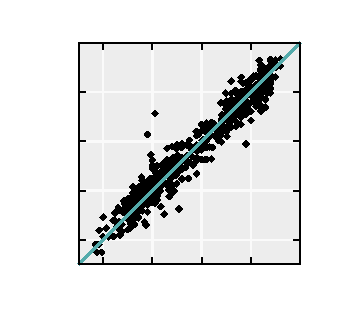
\includegraphics{gp/ms-sa-ph-corr}}%
    \gplfronttext
  \end{picture}%
\endgroup

				}
				\caption{\parbox[t]{0.43\textwidth}{
					$\widehat{\m{pH}} \sim \m{pH}$ \smallskip \\
					$(R^2)^{(\m{pH})} = 0.940$
					}}
				\label{sfig:gof-ph}
			\end{subfigure}
			\caption{Correlation diagrams plotting $\hat{y}$ on $y$ and the blue line representing the $\id$}
			\label{fig:gof}
		\end{figure*}

\section{Model Selection}
\label{sec:model-selection}
	
	\subsection{Calibration}
	\label{ssec:calibration}
	
		Figures \ref{sfig:calib-soc}, \ref{sfig:calib-n} and \ref{sfig:calib-ph} show the selected wavelengths highlighted in grey.
		One notes that the density of selected lightwaves varies strongly along the wavelengths for all three response variables, where $p^{(\m{SOC})}$ uses the most and $\m{pH}$ the lowest amount of predictors.
		
		For $p^{(\m{SOC})}$ and $p^{(\m{N})}$, we find that similar regions seeminlgy relevant for prediction, albeit the predictors for $p^{(\m{N})}$ appear to be slightly more evenly distributed along the whole domain of measured wavelengths. %Is that the correct term?.
		In the selected model for $p^{(\m{SOC})}$, predictors are highly concentrated in the regions from 1550 - 1650 $\unit{nm}$, 1790 - 1810 $\unit{nm}$, 1980 - 1990 $\unit{nm}$, around 2500 $\unit{nm}$ and between 2600 and 2672 $\unit{nm}$.
		
		The distribution of predictors for the $\m{pH}$ appears to be visibly distinct from the other two models.
		In particular, the lower-middle wavelengths seem to have more predictive power than for $p^{(\m{SOC})}$ and $p^{(\m{N})}$.
		
		Appendix \ref{sec:parameters} hosts the tables with the estimated parameters for the predictors for each model.
		It is noteworthy to inspect the values of the intercepts for each model.
		We find that these appear relatively close to 0 in case of $p^{\m{(SOC)}}$ and $p^{\m{(N)}}$.
		The $\m{pH}$ again sticks out as the value for its intercept is clearly placed in a mildly acidic range. % black coffee range ;)

				
	% subsection calibration

	\subsection{Goodness of Fit}
	\label{ssec:suitability}
	
		Figure \ref{fig:gof} displays the correlation diagrams introduced in \ref{ssec:model-validation} for each response variable together with the values for the $R^2$.
		Both indicate that our estimation and model selection to predict $\m{pH}$ are working best.
		Taking measurement error into account, an $R^2 = 0.940$ shows a good accordance between predictions by the model and the actual observed values.
		The clear pattern in diagram \ref{sfig:gof-ph} corroborates these findings.
		
		We have already seen on several occasions that $\m{pH}$ has to be treated slighted different from the other two response variables.
		The usual divergence between the patterns for the $\m{pH}$ and the other two response variables emerges here as well.
		$p^{\m{(SOC)}}$ and $p^{\m{(N)}}$ display not only lower values for $R^2$, but their correlation diagrams indicate a coherent divergence from the $\id$.
		
		Our predictions seem to underestimate the observed values for the upper third of the observed interval.
		This could be due to a lack of data, which are considerably scarcer in that region than in the regions where the fits appear good.
		Only less than 5 \% of the whole measurements lie in the upper tiers of both response variables.
		
		Another reason might be that the linear assumption is misplaced, by judging from the visual aspects of the scatter plot alone.
		As we have strong reason to maintain the linear hypothesis (\ref{ssec:nirs}) and taking into account that for most values the correlation seems even better than in the case of $\m{pH}$, we maintain that it is safe to assume higher measurement errors in as $p^{\m{(SOC)}}$ and $p^{\m{(N)}}$ increase, which in turn contributes to lower $R^2$ values.
		In sum, there is not sufficient evidence to reject the selected and estimated models at this point.
		
	% subsection suitability

% section model-selection
	\section{Simulation}
\label{sec:simulation}
	
	Applying the model selection algorithm to 1000 pseudo-observations of $p^{(\m{SOC})}$, we find that we underestimate the true $\m{SPSE}$ by a margin of $20.22$. 
	This is more than one standard deviation below the true value.
	As we decrease the number of used observations, this difference becomes increasingly and monotonously steeper as shown in the first column of table \ref{tab:sim-res}.
		
	\begin{table}[htb]
	\center
	\caption{simulation measurements, with true $\m{SPSE} = 172.85$}
	\label{tab:}
	\begin{tabular}{rrrrr}
		\hline
		$n$ & $m=1$ & $m=2$ & $m=3$ & $m=4$ \\
		\hline
		\hline
		\multirow{2}{*}{$533$}
		& $152.63$ & $192.47$ & $226.85$ & $250.58$ \\
		& $12.26$ & $12.94$ & $14.64$ & $15.23$ \\
		\hline
		\multirow{2}{*}{$500$}
		& $142.92$ & $180.17$ & $212.31$ & $237.15$ \\
		& $12.03$ & $12.63$ & $14.39$ & $14.81$ \\
		\hline
		\multirow{2}{*}{$400$}
		& $112.31$ & $138.81$ & $168.64$ & $184.81$ \\
		& $12.28$ & $11.26$ & $12.64$ & $13.28$ \\
		\hline
		\multirow{2}{*}{$300$}
		& --- & $104.82$ & $126.13$ & $139.38$ \\
		& --- & $10.44$ & $11.47$ & $11.93$ \\
		\hline
		\multirow{2}{*}{$200$}
		& --- & $66.34$ & $78.83$ & $89.46$ \\
		& --- & $10.15$ & $9.54$ & $10.08$ \\
		\hline
		\multirow{2}{*}{$100$}
		& --- & --- & --- & $40.45$ \\
		& --- & --- & --- & $9.10$ \\
		\hline
	\end{tabular}
\end{table}
	
	% report the results on the $\m{SPSE} - \widehat{\m{SPSE}} | m$
	Reducing the resolution in contrast leads to overestimation of the $\m{SPSE}$.
	Again, the difference between mean $\widehat{\m{SPSE}}$ and the true value is here monotone and increasing as can be seen in the first row of table \ref{tab:sim-res}.
	
	It is interesting to see that the standard deviation (and hence the variance) is increasing in $m$ but decreasing in $n$.
	Albeit the estimates for the $\m{SPSE}$ differ strongly, standard the deviation remains rather stable and within a close band around $12.5 \pm 3$
	
	The closest approximation to the true $\m{SPSE}$ is reached at 400 measurements and at a resolution of only a third of the original one.
	This indicates a strong dependence of the calibration on the original measuring setup.

% section simulation
	\section{Conclusion}
\label{sec:conclusion}
	
	

% section conclusion

	\begin{figure*}[h]
		\begin{subfigure}[b]{\textwidth}
			\centering
			% GNUPLOT: LaTeX picture with Postscript
\begingroup
  \makeatletter
  \providecommand\color[2][]{%
    \GenericError{(gnuplot) \space\space\space\@spaces}{%
      Package color not loaded in conjunction with
      terminal option `colourtext'%
    }{See the gnuplot documentation for explanation.%
    }{Either use 'blacktext' in gnuplot or load the package
      color.sty in LaTeX.}%
    \renewcommand\color[2][]{}%
  }%
  \providecommand\includegraphics[2][]{%
    \GenericError{(gnuplot) \space\space\space\@spaces}{%
      Package graphicx or graphics not loaded%
    }{See the gnuplot documentation for explanation.%
    }{The gnuplot epslatex terminal needs graphicx.sty or graphics.sty.}%
    \renewcommand\includegraphics[2][]{}%
  }%
  \providecommand\rotatebox[2]{#2}%
  \@ifundefined{ifGPcolor}{%
    \newif\ifGPcolor
    \GPcolorfalse
  }{}%
  \@ifundefined{ifGPblacktext}{%
    \newif\ifGPblacktext
    \GPblacktexttrue
  }{}%
  % define a \g@addto@macro without @ in the name:
  \let\gplgaddtomacro\g@addto@macro
  % define empty templates for all commands taking text:
  \gdef\gplbacktext{}%
  \gdef\gplfronttext{}%
  \makeatother
  \ifGPblacktext
    % no textcolor at all
    \def\colorrgb#1{}%
    \def\colorgray#1{}%
  \else
    % gray or color?
    \ifGPcolor
      \def\colorrgb#1{\color[rgb]{#1}}%
      \def\colorgray#1{\color[gray]{#1}}%
      \expandafter\def\csname LTw\endcsname{\color{white}}%
      \expandafter\def\csname LTb\endcsname{\color{black}}%
      \expandafter\def\csname LTa\endcsname{\color{black}}%
      \expandafter\def\csname LT0\endcsname{\color[rgb]{1,0,0}}%
      \expandafter\def\csname LT1\endcsname{\color[rgb]{0,1,0}}%
      \expandafter\def\csname LT2\endcsname{\color[rgb]{0,0,1}}%
      \expandafter\def\csname LT3\endcsname{\color[rgb]{1,0,1}}%
      \expandafter\def\csname LT4\endcsname{\color[rgb]{0,1,1}}%
      \expandafter\def\csname LT5\endcsname{\color[rgb]{1,1,0}}%
      \expandafter\def\csname LT6\endcsname{\color[rgb]{0,0,0}}%
      \expandafter\def\csname LT7\endcsname{\color[rgb]{1,0.3,0}}%
      \expandafter\def\csname LT8\endcsname{\color[rgb]{0.5,0.5,0.5}}%
    \else
      % gray
      \def\colorrgb#1{\color{black}}%
      \def\colorgray#1{\color[gray]{#1}}%
      \expandafter\def\csname LTw\endcsname{\color{white}}%
      \expandafter\def\csname LTb\endcsname{\color{black}}%
      \expandafter\def\csname LTa\endcsname{\color{black}}%
      \expandafter\def\csname LT0\endcsname{\color{black}}%
      \expandafter\def\csname LT1\endcsname{\color{black}}%
      \expandafter\def\csname LT2\endcsname{\color{black}}%
      \expandafter\def\csname LT3\endcsname{\color{black}}%
      \expandafter\def\csname LT4\endcsname{\color{black}}%
      \expandafter\def\csname LT5\endcsname{\color{black}}%
      \expandafter\def\csname LT6\endcsname{\color{black}}%
      \expandafter\def\csname LT7\endcsname{\color{black}}%
      \expandafter\def\csname LT8\endcsname{\color{black}}%
    \fi
  \fi
  \setlength{\unitlength}{0.0500bp}%
  \begin{picture}(7936.00,3400.00)%
    \gplgaddtomacro\gplbacktext{%
      \csname LTb\endcsname%
      \put(1078,704){\makebox(0,0)[r]{\strut{} 0.3}}%
      \csname LTb\endcsname%
      \put(1078,1190){\makebox(0,0)[r]{\strut{} 0.35}}%
      \csname LTb\endcsname%
      \put(1078,1676){\makebox(0,0)[r]{\strut{} 0.4}}%
      \csname LTb\endcsname%
      \put(1078,2163){\makebox(0,0)[r]{\strut{} 0.45}}%
      \csname LTb\endcsname%
      \put(1078,2649){\makebox(0,0)[r]{\strut{} 0.5}}%
      \csname LTb\endcsname%
      \put(1078,3135){\makebox(0,0)[r]{\strut{} 0.55}}%
      \csname LTb\endcsname%
      \put(1353,484){\makebox(0,0){\strut{} 1400}}%
      \csname LTb\endcsname%
      \put(2304,484){\makebox(0,0){\strut{} 1600}}%
      \csname LTb\endcsname%
      \put(3256,484){\makebox(0,0){\strut{} 1800}}%
      \csname LTb\endcsname%
      \put(4208,484){\makebox(0,0){\strut{} 2000}}%
      \csname LTb\endcsname%
      \put(5160,484){\makebox(0,0){\strut{} 2200}}%
      \csname LTb\endcsname%
      \put(6111,484){\makebox(0,0){\strut{} 2400}}%
      \csname LTb\endcsname%
      \put(7063,484){\makebox(0,0){\strut{} 2600}}%
      \put(176,1919){\rotatebox{-270}{\makebox(0,0){\strut{}$-\lg \varrho(\lambda)$}}}%
      \put(4374,154){\makebox(0,0){\strut{}$\lambda \ [\m{nm}]$}}%
    }%
    \gplgaddtomacro\gplfronttext{%
      \csname LTb\endcsname%
      \put(6587,2892){\makebox(0,0)[l]{\strut{}SOC}}%
    }%
    \gplbacktext
    \put(0,0){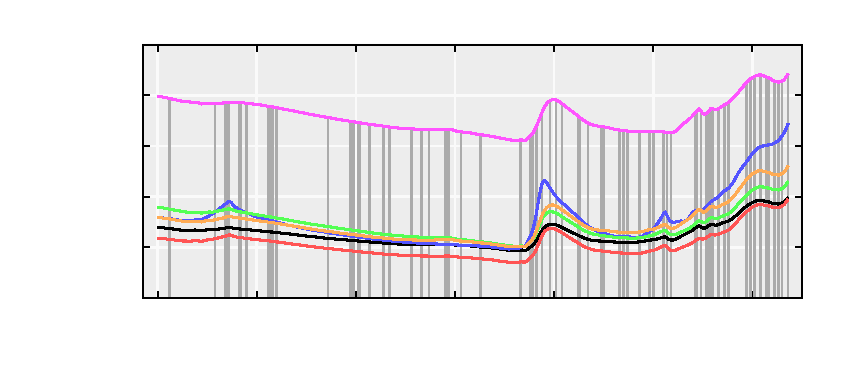
\includegraphics{gp/ms-sa-soc-spec-rnd}}%
    \gplfronttext
  \end{picture}%
\endgroup

			\caption{SOC}
			\label{fig:}
		\end{subfigure}
		
		\begin{subfigure}[b]{\textwidth}
			\centering
			% GNUPLOT: LaTeX picture with Postscript
\begingroup
  \makeatletter
  \providecommand\color[2][]{%
    \GenericError{(gnuplot) \space\space\space\@spaces}{%
      Package color not loaded in conjunction with
      terminal option `colourtext'%
    }{See the gnuplot documentation for explanation.%
    }{Either use 'blacktext' in gnuplot or load the package
      color.sty in LaTeX.}%
    \renewcommand\color[2][]{}%
  }%
  \providecommand\includegraphics[2][]{%
    \GenericError{(gnuplot) \space\space\space\@spaces}{%
      Package graphicx or graphics not loaded%
    }{See the gnuplot documentation for explanation.%
    }{The gnuplot epslatex terminal needs graphicx.sty or graphics.sty.}%
    \renewcommand\includegraphics[2][]{}%
  }%
  \providecommand\rotatebox[2]{#2}%
  \@ifundefined{ifGPcolor}{%
    \newif\ifGPcolor
    \GPcolorfalse
  }{}%
  \@ifundefined{ifGPblacktext}{%
    \newif\ifGPblacktext
    \GPblacktexttrue
  }{}%
  % define a \g@addto@macro without @ in the name:
  \let\gplgaddtomacro\g@addto@macro
  % define empty templates for all commands taking text:
  \gdef\gplbacktext{}%
  \gdef\gplfronttext{}%
  \makeatother
  \ifGPblacktext
    % no textcolor at all
    \def\colorrgb#1{}%
    \def\colorgray#1{}%
  \else
    % gray or color?
    \ifGPcolor
      \def\colorrgb#1{\color[rgb]{#1}}%
      \def\colorgray#1{\color[gray]{#1}}%
      \expandafter\def\csname LTw\endcsname{\color{white}}%
      \expandafter\def\csname LTb\endcsname{\color{black}}%
      \expandafter\def\csname LTa\endcsname{\color{black}}%
      \expandafter\def\csname LT0\endcsname{\color[rgb]{1,0,0}}%
      \expandafter\def\csname LT1\endcsname{\color[rgb]{0,1,0}}%
      \expandafter\def\csname LT2\endcsname{\color[rgb]{0,0,1}}%
      \expandafter\def\csname LT3\endcsname{\color[rgb]{1,0,1}}%
      \expandafter\def\csname LT4\endcsname{\color[rgb]{0,1,1}}%
      \expandafter\def\csname LT5\endcsname{\color[rgb]{1,1,0}}%
      \expandafter\def\csname LT6\endcsname{\color[rgb]{0,0,0}}%
      \expandafter\def\csname LT7\endcsname{\color[rgb]{1,0.3,0}}%
      \expandafter\def\csname LT8\endcsname{\color[rgb]{0.5,0.5,0.5}}%
    \else
      % gray
      \def\colorrgb#1{\color{black}}%
      \def\colorgray#1{\color[gray]{#1}}%
      \expandafter\def\csname LTw\endcsname{\color{white}}%
      \expandafter\def\csname LTb\endcsname{\color{black}}%
      \expandafter\def\csname LTa\endcsname{\color{black}}%
      \expandafter\def\csname LT0\endcsname{\color{black}}%
      \expandafter\def\csname LT1\endcsname{\color{black}}%
      \expandafter\def\csname LT2\endcsname{\color{black}}%
      \expandafter\def\csname LT3\endcsname{\color{black}}%
      \expandafter\def\csname LT4\endcsname{\color{black}}%
      \expandafter\def\csname LT5\endcsname{\color{black}}%
      \expandafter\def\csname LT6\endcsname{\color{black}}%
      \expandafter\def\csname LT7\endcsname{\color{black}}%
      \expandafter\def\csname LT8\endcsname{\color{black}}%
    \fi
  \fi
  \setlength{\unitlength}{0.0500bp}%
  \begin{picture}(7936.00,3400.00)%
    \gplgaddtomacro\gplbacktext{%
      \csname LTb\endcsname%
      \put(1078,704){\makebox(0,0)[r]{\strut{} 0.3}}%
      \csname LTb\endcsname%
      \put(1078,1190){\makebox(0,0)[r]{\strut{} 0.35}}%
      \csname LTb\endcsname%
      \put(1078,1676){\makebox(0,0)[r]{\strut{} 0.4}}%
      \csname LTb\endcsname%
      \put(1078,2163){\makebox(0,0)[r]{\strut{} 0.45}}%
      \csname LTb\endcsname%
      \put(1078,2649){\makebox(0,0)[r]{\strut{} 0.5}}%
      \csname LTb\endcsname%
      \put(1078,3135){\makebox(0,0)[r]{\strut{} 0.55}}%
      \csname LTb\endcsname%
      \put(1353,484){\makebox(0,0){\strut{} 1400}}%
      \csname LTb\endcsname%
      \put(2304,484){\makebox(0,0){\strut{} 1600}}%
      \csname LTb\endcsname%
      \put(3256,484){\makebox(0,0){\strut{} 1800}}%
      \csname LTb\endcsname%
      \put(4208,484){\makebox(0,0){\strut{} 2000}}%
      \csname LTb\endcsname%
      \put(5160,484){\makebox(0,0){\strut{} 2200}}%
      \csname LTb\endcsname%
      \put(6111,484){\makebox(0,0){\strut{} 2400}}%
      \csname LTb\endcsname%
      \put(7063,484){\makebox(0,0){\strut{} 2600}}%
      \put(176,1919){\rotatebox{-270}{\makebox(0,0){\strut{}$-\lg \varrho(\lambda)$}}}%
      \put(4374,154){\makebox(0,0){\strut{}$\lambda \ [\m{nm}]$}}%
    }%
    \gplgaddtomacro\gplfronttext{%
      \csname LTb\endcsname%
      \put(6587,2892){\makebox(0,0)[r]{\strut{}$P^\m{(N)}$}}%
    }%
    \gplbacktext
    \put(0,0){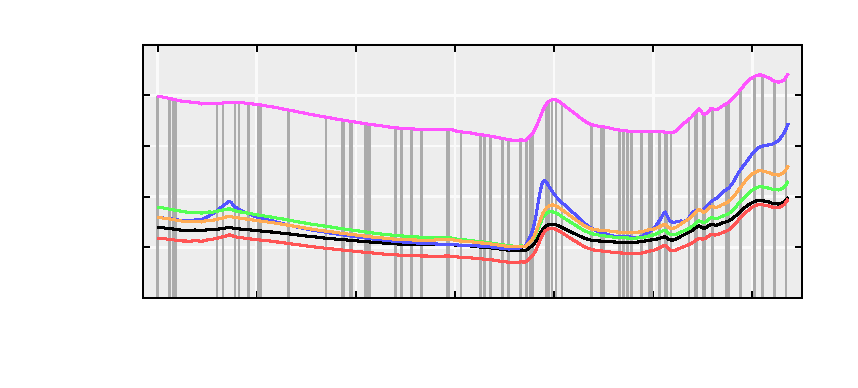
\includegraphics{gp/ms-sa-n-spec-rnd}}%
    \gplfronttext
  \end{picture}%
\endgroup

			\caption{N}
			\label{fig:}
		\end{subfigure}

		\begin{subfigure}[b]{\textwidth}
			\centering
			% GNUPLOT: LaTeX picture with Postscript
\begingroup
  \makeatletter
  \providecommand\color[2][]{%
    \GenericError{(gnuplot) \space\space\space\@spaces}{%
      Package color not loaded in conjunction with
      terminal option `colourtext'%
    }{See the gnuplot documentation for explanation.%
    }{Either use 'blacktext' in gnuplot or load the package
      color.sty in LaTeX.}%
    \renewcommand\color[2][]{}%
  }%
  \providecommand\includegraphics[2][]{%
    \GenericError{(gnuplot) \space\space\space\@spaces}{%
      Package graphicx or graphics not loaded%
    }{See the gnuplot documentation for explanation.%
    }{The gnuplot epslatex terminal needs graphicx.sty or graphics.sty.}%
    \renewcommand\includegraphics[2][]{}%
  }%
  \providecommand\rotatebox[2]{#2}%
  \@ifundefined{ifGPcolor}{%
    \newif\ifGPcolor
    \GPcolorfalse
  }{}%
  \@ifundefined{ifGPblacktext}{%
    \newif\ifGPblacktext
    \GPblacktexttrue
  }{}%
  % define a \g@addto@macro without @ in the name:
  \let\gplgaddtomacro\g@addto@macro
  % define empty templates for all commands taking text:
  \gdef\gplbacktext{}%
  \gdef\gplfronttext{}%
  \makeatother
  \ifGPblacktext
    % no textcolor at all
    \def\colorrgb#1{}%
    \def\colorgray#1{}%
  \else
    % gray or color?
    \ifGPcolor
      \def\colorrgb#1{\color[rgb]{#1}}%
      \def\colorgray#1{\color[gray]{#1}}%
      \expandafter\def\csname LTw\endcsname{\color{white}}%
      \expandafter\def\csname LTb\endcsname{\color{black}}%
      \expandafter\def\csname LTa\endcsname{\color{black}}%
      \expandafter\def\csname LT0\endcsname{\color[rgb]{1,0,0}}%
      \expandafter\def\csname LT1\endcsname{\color[rgb]{0,1,0}}%
      \expandafter\def\csname LT2\endcsname{\color[rgb]{0,0,1}}%
      \expandafter\def\csname LT3\endcsname{\color[rgb]{1,0,1}}%
      \expandafter\def\csname LT4\endcsname{\color[rgb]{0,1,1}}%
      \expandafter\def\csname LT5\endcsname{\color[rgb]{1,1,0}}%
      \expandafter\def\csname LT6\endcsname{\color[rgb]{0,0,0}}%
      \expandafter\def\csname LT7\endcsname{\color[rgb]{1,0.3,0}}%
      \expandafter\def\csname LT8\endcsname{\color[rgb]{0.5,0.5,0.5}}%
    \else
      % gray
      \def\colorrgb#1{\color{black}}%
      \def\colorgray#1{\color[gray]{#1}}%
      \expandafter\def\csname LTw\endcsname{\color{white}}%
      \expandafter\def\csname LTb\endcsname{\color{black}}%
      \expandafter\def\csname LTa\endcsname{\color{black}}%
      \expandafter\def\csname LT0\endcsname{\color{black}}%
      \expandafter\def\csname LT1\endcsname{\color{black}}%
      \expandafter\def\csname LT2\endcsname{\color{black}}%
      \expandafter\def\csname LT3\endcsname{\color{black}}%
      \expandafter\def\csname LT4\endcsname{\color{black}}%
      \expandafter\def\csname LT5\endcsname{\color{black}}%
      \expandafter\def\csname LT6\endcsname{\color{black}}%
      \expandafter\def\csname LT7\endcsname{\color{black}}%
      \expandafter\def\csname LT8\endcsname{\color{black}}%
    \fi
  \fi
  \setlength{\unitlength}{0.0500bp}%
  \begin{picture}(7936.00,3400.00)%
    \gplgaddtomacro\gplbacktext{%
      \csname LTb\endcsname%
      \put(1078,704){\makebox(0,0)[r]{\strut{} 0.3}}%
      \csname LTb\endcsname%
      \put(1078,1190){\makebox(0,0)[r]{\strut{} 0.35}}%
      \csname LTb\endcsname%
      \put(1078,1676){\makebox(0,0)[r]{\strut{} 0.4}}%
      \csname LTb\endcsname%
      \put(1078,2163){\makebox(0,0)[r]{\strut{} 0.45}}%
      \csname LTb\endcsname%
      \put(1078,2649){\makebox(0,0)[r]{\strut{} 0.5}}%
      \csname LTb\endcsname%
      \put(1078,3135){\makebox(0,0)[r]{\strut{} 0.55}}%
      \csname LTb\endcsname%
      \put(1353,484){\makebox(0,0){\strut{} 1400}}%
      \csname LTb\endcsname%
      \put(2304,484){\makebox(0,0){\strut{} 1600}}%
      \csname LTb\endcsname%
      \put(3256,484){\makebox(0,0){\strut{} 1800}}%
      \csname LTb\endcsname%
      \put(4208,484){\makebox(0,0){\strut{} 2000}}%
      \csname LTb\endcsname%
      \put(5160,484){\makebox(0,0){\strut{} 2200}}%
      \csname LTb\endcsname%
      \put(6111,484){\makebox(0,0){\strut{} 2400}}%
      \csname LTb\endcsname%
      \put(7063,484){\makebox(0,0){\strut{} 2600}}%
      \put(176,1919){\rotatebox{-270}{\makebox(0,0){\strut{}$-\lg \varrho(\lambda)$}}}%
      \put(4374,154){\makebox(0,0){\strut{}$\lambda \ [\m{nm}]$}}%
    }%
    \gplgaddtomacro\gplfronttext{%
      \csname LTb\endcsname%
      \put(6587,2892){\makebox(0,0)[l]{\strut{}pH}}%
    }%
    \gplbacktext
    \put(0,0){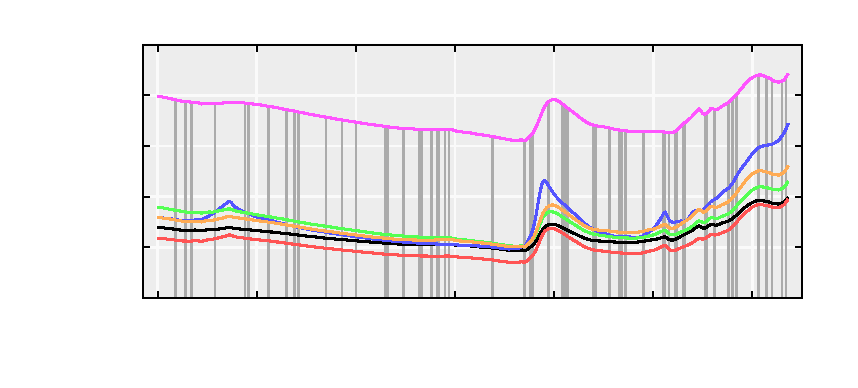
\includegraphics{gp/ms-sa-ph-spec-rnd}}%
    \gplfronttext
  \end{picture}%
\endgroup

			\caption{pH}
			\label{fig:}
		\end{subfigure}
	\end{figure*}


	\begin{figure*}[h]
		\center
		\begin{subfigure}[b]{0.33\textwidth}
			\centerline{
				% GNUPLOT: LaTeX picture with Postscript
\begingroup
  \makeatletter
  \providecommand\color[2][]{%
    \GenericError{(gnuplot) \space\space\space\@spaces}{%
      Package color not loaded in conjunction with
      terminal option `colourtext'%
    }{See the gnuplot documentation for explanation.%
    }{Either use 'blacktext' in gnuplot or load the package
      color.sty in LaTeX.}%
    \renewcommand\color[2][]{}%
  }%
  \providecommand\includegraphics[2][]{%
    \GenericError{(gnuplot) \space\space\space\@spaces}{%
      Package graphicx or graphics not loaded%
    }{See the gnuplot documentation for explanation.%
    }{The gnuplot epslatex terminal needs graphicx.sty or graphics.sty.}%
    \renewcommand\includegraphics[2][]{}%
  }%
  \providecommand\rotatebox[2]{#2}%
  \@ifundefined{ifGPcolor}{%
    \newif\ifGPcolor
    \GPcolorfalse
  }{}%
  \@ifundefined{ifGPblacktext}{%
    \newif\ifGPblacktext
    \GPblacktexttrue
  }{}%
  % define a \g@addto@macro without @ in the name:
  \let\gplgaddtomacro\g@addto@macro
  % define empty templates for all commands taking text:
  \gdef\gplbacktext{}%
  \gdef\gplfronttext{}%
  \makeatother
  \ifGPblacktext
    % no textcolor at all
    \def\colorrgb#1{}%
    \def\colorgray#1{}%
  \else
    % gray or color?
    \ifGPcolor
      \def\colorrgb#1{\color[rgb]{#1}}%
      \def\colorgray#1{\color[gray]{#1}}%
      \expandafter\def\csname LTw\endcsname{\color{white}}%
      \expandafter\def\csname LTb\endcsname{\color{black}}%
      \expandafter\def\csname LTa\endcsname{\color{black}}%
      \expandafter\def\csname LT0\endcsname{\color[rgb]{1,0,0}}%
      \expandafter\def\csname LT1\endcsname{\color[rgb]{0,1,0}}%
      \expandafter\def\csname LT2\endcsname{\color[rgb]{0,0,1}}%
      \expandafter\def\csname LT3\endcsname{\color[rgb]{1,0,1}}%
      \expandafter\def\csname LT4\endcsname{\color[rgb]{0,1,1}}%
      \expandafter\def\csname LT5\endcsname{\color[rgb]{1,1,0}}%
      \expandafter\def\csname LT6\endcsname{\color[rgb]{0,0,0}}%
      \expandafter\def\csname LT7\endcsname{\color[rgb]{1,0.3,0}}%
      \expandafter\def\csname LT8\endcsname{\color[rgb]{0.5,0.5,0.5}}%
    \else
      % gray
      \def\colorrgb#1{\color{black}}%
      \def\colorgray#1{\color[gray]{#1}}%
      \expandafter\def\csname LTw\endcsname{\color{white}}%
      \expandafter\def\csname LTb\endcsname{\color{black}}%
      \expandafter\def\csname LTa\endcsname{\color{black}}%
      \expandafter\def\csname LT0\endcsname{\color{black}}%
      \expandafter\def\csname LT1\endcsname{\color{black}}%
      \expandafter\def\csname LT2\endcsname{\color{black}}%
      \expandafter\def\csname LT3\endcsname{\color{black}}%
      \expandafter\def\csname LT4\endcsname{\color{black}}%
      \expandafter\def\csname LT5\endcsname{\color{black}}%
      \expandafter\def\csname LT6\endcsname{\color{black}}%
      \expandafter\def\csname LT7\endcsname{\color{black}}%
      \expandafter\def\csname LT8\endcsname{\color{black}}%
    \fi
  \fi
  \setlength{\unitlength}{0.0500bp}%
  \begin{picture}(3118.00,2834.00)%
    \gplgaddtomacro\gplbacktext{%
      \csname LTb\endcsname%
      \put(594,688){\makebox(0,0)[r]{\strut{} 0}}%
      \csname LTb\endcsname%
      \put(594,1051){\makebox(0,0)[r]{\strut{} 2}}%
      \csname LTb\endcsname%
      \put(594,1414){\makebox(0,0)[r]{\strut{} 4}}%
      \csname LTb\endcsname%
      \put(594,1777){\makebox(0,0)[r]{\strut{} 6}}%
      \csname LTb\endcsname%
      \put(594,2139){\makebox(0,0)[r]{\strut{} 8}}%
      \csname LTb\endcsname%
      \put(594,2502){\makebox(0,0)[r]{\strut{} 10}}%
      \csname LTb\endcsname%
      \put(907,287){\makebox(0,0){\strut{} 0}}%
      \csname LTb\endcsname%
      \put(1270,287){\makebox(0,0){\strut{} 2}}%
      \csname LTb\endcsname%
      \put(1633,287){\makebox(0,0){\strut{} 4}}%
      \csname LTb\endcsname%
      \put(1996,287){\makebox(0,0){\strut{} 6}}%
      \csname LTb\endcsname%
      \put(2358,287){\makebox(0,0){\strut{} 8}}%
      \csname LTb\endcsname%
      \put(2721,287){\makebox(0,0){\strut{} 10}}%
    }%
    \gplgaddtomacro\gplfronttext{%
      \csname LTb\endcsname%
      \put(1089,2139){\makebox(0,0)[l]{\strut{}SOC}}%
    }%
    \gplbacktext
    \put(0,0){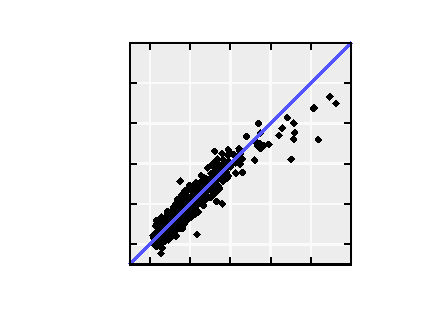
\includegraphics{gp/ms-sa-soc-corr}}%
    \gplfronttext
  \end{picture}%
\endgroup

			}
			\caption{SOC}
		\end{subfigure}
		\begin{subfigure}[b]{0.33\textwidth}
			\centerline{
				% GNUPLOT: LaTeX picture with Postscript
\begingroup
  \makeatletter
  \providecommand\color[2][]{%
    \GenericError{(gnuplot) \space\space\space\@spaces}{%
      Package color not loaded in conjunction with
      terminal option `colourtext'%
    }{See the gnuplot documentation for explanation.%
    }{Either use 'blacktext' in gnuplot or load the package
      color.sty in LaTeX.}%
    \renewcommand\color[2][]{}%
  }%
  \providecommand\includegraphics[2][]{%
    \GenericError{(gnuplot) \space\space\space\@spaces}{%
      Package graphicx or graphics not loaded%
    }{See the gnuplot documentation for explanation.%
    }{The gnuplot epslatex terminal needs graphicx.sty or graphics.sty.}%
    \renewcommand\includegraphics[2][]{}%
  }%
  \providecommand\rotatebox[2]{#2}%
  \@ifundefined{ifGPcolor}{%
    \newif\ifGPcolor
    \GPcolorfalse
  }{}%
  \@ifundefined{ifGPblacktext}{%
    \newif\ifGPblacktext
    \GPblacktexttrue
  }{}%
  % define a \g@addto@macro without @ in the name:
  \let\gplgaddtomacro\g@addto@macro
  % define empty templates for all commands taking text:
  \gdef\gplbacktext{}%
  \gdef\gplfronttext{}%
  \makeatother
  \ifGPblacktext
    % no textcolor at all
    \def\colorrgb#1{}%
    \def\colorgray#1{}%
  \else
    % gray or color?
    \ifGPcolor
      \def\colorrgb#1{\color[rgb]{#1}}%
      \def\colorgray#1{\color[gray]{#1}}%
      \expandafter\def\csname LTw\endcsname{\color{white}}%
      \expandafter\def\csname LTb\endcsname{\color{black}}%
      \expandafter\def\csname LTa\endcsname{\color{black}}%
      \expandafter\def\csname LT0\endcsname{\color[rgb]{1,0,0}}%
      \expandafter\def\csname LT1\endcsname{\color[rgb]{0,1,0}}%
      \expandafter\def\csname LT2\endcsname{\color[rgb]{0,0,1}}%
      \expandafter\def\csname LT3\endcsname{\color[rgb]{1,0,1}}%
      \expandafter\def\csname LT4\endcsname{\color[rgb]{0,1,1}}%
      \expandafter\def\csname LT5\endcsname{\color[rgb]{1,1,0}}%
      \expandafter\def\csname LT6\endcsname{\color[rgb]{0,0,0}}%
      \expandafter\def\csname LT7\endcsname{\color[rgb]{1,0.3,0}}%
      \expandafter\def\csname LT8\endcsname{\color[rgb]{0.5,0.5,0.5}}%
    \else
      % gray
      \def\colorrgb#1{\color{black}}%
      \def\colorgray#1{\color[gray]{#1}}%
      \expandafter\def\csname LTw\endcsname{\color{white}}%
      \expandafter\def\csname LTb\endcsname{\color{black}}%
      \expandafter\def\csname LTa\endcsname{\color{black}}%
      \expandafter\def\csname LT0\endcsname{\color{black}}%
      \expandafter\def\csname LT1\endcsname{\color{black}}%
      \expandafter\def\csname LT2\endcsname{\color{black}}%
      \expandafter\def\csname LT3\endcsname{\color{black}}%
      \expandafter\def\csname LT4\endcsname{\color{black}}%
      \expandafter\def\csname LT5\endcsname{\color{black}}%
      \expandafter\def\csname LT6\endcsname{\color{black}}%
      \expandafter\def\csname LT7\endcsname{\color{black}}%
      \expandafter\def\csname LT8\endcsname{\color{black}}%
    \fi
  \fi
  \setlength{\unitlength}{0.0500bp}%
  \begin{picture}(3968.00,2834.00)%
    \gplgaddtomacro\gplbacktext{%
      \csname LTb\endcsname%
      \put(1018,677){\makebox(0,0)[r]{\strut{} 0}}%
      \csname LTb\endcsname%
      \put(1018,1150){\makebox(0,0)[r]{\strut{} 0.2}}%
      \csname LTb\endcsname%
      \put(1018,1623){\makebox(0,0)[r]{\strut{} 0.4}}%
      \csname LTb\endcsname%
      \put(1018,2096){\makebox(0,0)[r]{\strut{} 0.6}}%
      \csname LTb\endcsname%
      \put(1018,2569){\makebox(0,0)[r]{\strut{} 0.8}}%
      \csname LTb\endcsname%
      \put(1387,220){\makebox(0,0){\strut{} 0}}%
      \csname LTb\endcsname%
      \put(1860,220){\makebox(0,0){\strut{} 0.2}}%
      \csname LTb\endcsname%
      \put(2333,220){\makebox(0,0){\strut{} 0.4}}%
      \csname LTb\endcsname%
      \put(2806,220){\makebox(0,0){\strut{} 0.6}}%
      \csname LTb\endcsname%
      \put(3279,220){\makebox(0,0){\strut{} 0.8}}%
    }%
    \gplgaddtomacro\gplfronttext{%
      \csname LTb\endcsname%
      \put(1469,2250){\makebox(0,0)[l]{\strut{}$P^\m{(N)}$}}%
    }%
    \gplbacktext
    \put(0,0){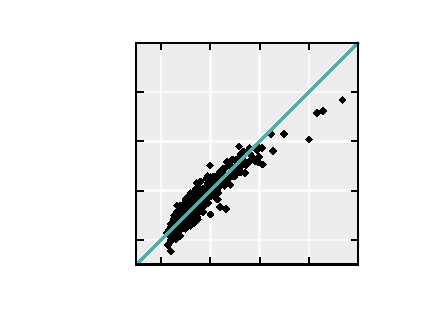
\includegraphics{gp/ms-sa-n-corr}}%
    \gplfronttext
  \end{picture}%
\endgroup

			}
			\caption{N}
		\end{subfigure}
		\begin{subfigure}[b]{0.33\textwidth}
			\centerline{
				% GNUPLOT: LaTeX picture with Postscript
\begingroup
  \makeatletter
  \providecommand\color[2][]{%
    \GenericError{(gnuplot) \space\space\space\@spaces}{%
      Package color not loaded in conjunction with
      terminal option `colourtext'%
    }{See the gnuplot documentation for explanation.%
    }{Either use 'blacktext' in gnuplot or load the package
      color.sty in LaTeX.}%
    \renewcommand\color[2][]{}%
  }%
  \providecommand\includegraphics[2][]{%
    \GenericError{(gnuplot) \space\space\space\@spaces}{%
      Package graphicx or graphics not loaded%
    }{See the gnuplot documentation for explanation.%
    }{The gnuplot epslatex terminal needs graphicx.sty or graphics.sty.}%
    \renewcommand\includegraphics[2][]{}%
  }%
  \providecommand\rotatebox[2]{#2}%
  \@ifundefined{ifGPcolor}{%
    \newif\ifGPcolor
    \GPcolorfalse
  }{}%
  \@ifundefined{ifGPblacktext}{%
    \newif\ifGPblacktext
    \GPblacktexttrue
  }{}%
  % define a \g@addto@macro without @ in the name:
  \let\gplgaddtomacro\g@addto@macro
  % define empty templates for all commands taking text:
  \gdef\gplbacktext{}%
  \gdef\gplfronttext{}%
  \makeatother
  \ifGPblacktext
    % no textcolor at all
    \def\colorrgb#1{}%
    \def\colorgray#1{}%
  \else
    % gray or color?
    \ifGPcolor
      \def\colorrgb#1{\color[rgb]{#1}}%
      \def\colorgray#1{\color[gray]{#1}}%
      \expandafter\def\csname LTw\endcsname{\color{white}}%
      \expandafter\def\csname LTb\endcsname{\color{black}}%
      \expandafter\def\csname LTa\endcsname{\color{black}}%
      \expandafter\def\csname LT0\endcsname{\color[rgb]{1,0,0}}%
      \expandafter\def\csname LT1\endcsname{\color[rgb]{0,1,0}}%
      \expandafter\def\csname LT2\endcsname{\color[rgb]{0,0,1}}%
      \expandafter\def\csname LT3\endcsname{\color[rgb]{1,0,1}}%
      \expandafter\def\csname LT4\endcsname{\color[rgb]{0,1,1}}%
      \expandafter\def\csname LT5\endcsname{\color[rgb]{1,1,0}}%
      \expandafter\def\csname LT6\endcsname{\color[rgb]{0,0,0}}%
      \expandafter\def\csname LT7\endcsname{\color[rgb]{1,0.3,0}}%
      \expandafter\def\csname LT8\endcsname{\color[rgb]{0.5,0.5,0.5}}%
    \else
      % gray
      \def\colorrgb#1{\color{black}}%
      \def\colorgray#1{\color[gray]{#1}}%
      \expandafter\def\csname LTw\endcsname{\color{white}}%
      \expandafter\def\csname LTb\endcsname{\color{black}}%
      \expandafter\def\csname LTa\endcsname{\color{black}}%
      \expandafter\def\csname LT0\endcsname{\color{black}}%
      \expandafter\def\csname LT1\endcsname{\color{black}}%
      \expandafter\def\csname LT2\endcsname{\color{black}}%
      \expandafter\def\csname LT3\endcsname{\color{black}}%
      \expandafter\def\csname LT4\endcsname{\color{black}}%
      \expandafter\def\csname LT5\endcsname{\color{black}}%
      \expandafter\def\csname LT6\endcsname{\color{black}}%
      \expandafter\def\csname LT7\endcsname{\color{black}}%
      \expandafter\def\csname LT8\endcsname{\color{black}}%
    \fi
  \fi
  \setlength{\unitlength}{0.0500bp}%
  \begin{picture}(3968.00,2834.00)%
    \gplgaddtomacro\gplbacktext{%
      \csname LTb\endcsname%
      \put(886,677){\makebox(0,0)[r]{\strut{} 4}}%
      \csname LTb\endcsname%
      \put(886,1150){\makebox(0,0)[r]{\strut{} 5}}%
      \csname LTb\endcsname%
      \put(886,1623){\makebox(0,0)[r]{\strut{} 6}}%
      \csname LTb\endcsname%
      \put(886,2096){\makebox(0,0)[r]{\strut{} 7}}%
      \csname LTb\endcsname%
      \put(886,2569){\makebox(0,0)[r]{\strut{} 8}}%
      \csname LTb\endcsname%
      \put(1255,220){\makebox(0,0){\strut{} 4}}%
      \csname LTb\endcsname%
      \put(1728,220){\makebox(0,0){\strut{} 5}}%
      \csname LTb\endcsname%
      \put(2201,220){\makebox(0,0){\strut{} 6}}%
      \csname LTb\endcsname%
      \put(2674,220){\makebox(0,0){\strut{} 7}}%
      \csname LTb\endcsname%
      \put(3147,220){\makebox(0,0){\strut{} 8}}%
    }%
    \gplgaddtomacro\gplfronttext{%
      \csname LTb\endcsname%
      \put(1349,2191){\makebox(0,0)[l]{\strut{}pH}}%
    }%
    \gplbacktext
    \put(0,0){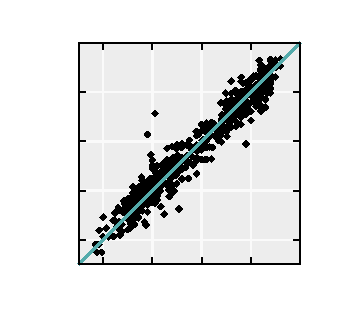
\includegraphics{gp/ms-sa-ph-corr}}%
    \gplfronttext
  \end{picture}%
\endgroup

			}
			\caption{pH}
		\end{subfigure}
		\caption{correlation}
	\end{figure*}

	\bibliography{}
	
	\appendix
	\onecolumn
	\pagenumbering{roman}
	\section{Prediction Parameters}
\label{sec:parameters}
	
	\begin{table}[ht]
		\center
		\caption{Estimated model parameters of $P^\m{SOC}$ on selected model}
		\setlength{\extrarowheight}{4pt}
		\begin{tabular}{rr|rr|rr|rr}
			\hline
			$\lambda_i \ [\m{nm}]$ & $\beta^\m{(SOC)}_i$ & $\lambda_i \ [\m{nm}]$ & $\beta^\m{(SOC)}_i$ & $\lambda_i \ [\m{nm}]$ & $\beta^\m{(SOC)}_i$ & $\lambda_i \ [\m{nm}]$ & $\beta^\m{(SOC)}_i$ \\
			\hline
			\hline
			--- & -1.37 & 1696 & -1166.38 & 2108 & -1382.98 & 2460 & -361.83\\
1400 & 826.04 & 1744 & 1424.94 & 2120 & 1645.94 & 2484 & 2332.83\\
1424 & -1324.59 & 1788 & -2087.12 & 2144 & 3204.64 & 2488 & -2705.44\\
1436 & -642.72 & 1792 & 1898.5 & 2148 & -2621.19 & 2496 & 1771.59\\
1464 & -980.9 & 1800 & -1558.26 & 2180 & -613.88 & 2508 & -4389.54\\
1468 & 1201.95 & 1808 & 1438.45 & 2192 & 1799.45 & 2512 & 3378.91\\
1516 & 1117.94 & 1832 & 2504.93 & 2204 & -2726.43 & 2516 & -2699.09\\
1536 & 2049.48 & 1836 & -1326.38 & 2216 & 1810.36 & 2520 & 2754.49\\
1540 & -2041.89 & 1856 & -2577.96 & 2240 & -1500.87 & 2548 & -2761.22\\
1544 & 1154.3 & 1880 & 1275.66 & 2248 & 1717.8 & 2552 & 2224.56\\
1552 & -1298.43 & 1912 & -2522.78 & 2272 & -1654.19 & 2580 & 1071.07\\
1556 & 2252.06 & 1932 & 1325.29 & 2304 & 1191.13 & 2600 & -1589.8\\
1560 & -2277.97 & 1948 & 1592.08 & 2332 & -2318.41 & 2620 & 1163.85\\
1580 & -950.58 & 1980 & -1994.92 & 2340 & 3079.92 & 2628 & 1414.16\\
1592 & -1627.88 & 1984 & 3827.51 & 2348 & -1970.47 & 2632 & -2540.03\\
1596 & 1697.58 & 1988 & -3669.48 & 2352 & -2222.55 & 2636 & 1154.67\\
1612 & 857.87 & 2012 & 1860.69 & 2356 & 3881.99 & 2648 & -1231.84\\
1624 & 1472.47 & 2052 & -2273.32 & 2420 & -1023.57 & 2672 & 771.23\\
1628 & -2702.99 & 2072 & 3197.8 & 2432 & 2104.87 & & \\
1632 & 3339.95 & 2092 & -1376.49 & 2436 & -2772.6 & & \\
1636 & -1430.86 & 2100 & -1309.64 & 2440 & 1443.54 & & \\

			\hline \\
		\end{tabular}
	\end{table}

	\begin{table}[H]
		\center
		\caption{Estimated model parameters of $P^\m{N}$ on selected model}
		\setlength{\extrarowheight}{2.2pt}
		\begin{tabular}{rr|rr|rr|rr}
			\hline
			$\lambda_i \ [\m{nm}]$ & $\beta^\m{(N)}_i$ & $\lambda_i \ [\m{nm}]$ & $\beta^\m{(N)}_i$ & $\lambda_i \ [\m{nm}]$ & $\beta^\m{(N)}_i$ & $\lambda_i \ [\m{nm}]$ & $\beta^\m{(N)}_i$ \\
			\hline
			\hline
			--- & -0.03 & 1824 & -322.95 & 2176 & -55.01 & 2480 & 146.55\\
1432 & 57.15 & 1828 & 264.85 & 2188 & 68.57 & 2484 & -124.23\\
1436 & -96.58 & 1860 & -89.78 & 2208 & -198.14 & 2500 & 223.14\\
1452 & -49.73 & 1904 & 91.91 & 2216 & 182.95 & 2504 & -279.93\\
1468 & 48.52 & 1912 & -207.41 & 2276 & -269.65 & 2520 & 55.77\\
1476 & -83.09 & 1924 & -117.17 & 2280 & 138.84 & 2536 & 93.88\\
1480 & 79.57 & 1932 & 120.37 & 2300 & 125.9 & 2540 & -101.02\\
1520 & 76.62 & 1948 & 138.91 & 2332 & -140.59 & 2548 & -226.8\\
1536 & 41.5 & 1988 & -96.24 & 2336 & 135.15 & 2552 & 202.85\\
1556 & 89.72 & 2012 & 123.7 & 2344 & 182.6 & 2576 & 79.15\\
1560 & -109.73 & 2052 & -193.08 & 2348 & -315.73 & 2596 & -50.8\\
1580 & -103.8 & 2060 & 125.31 & 2356 & 175.07 & 2604 & -67.93\\
1608 & 73.7 & 2108 & -191.7 & 2420 & -71.9 & 2620 & 86.74\\
1668 & -71.2 & 2136 & 92.38 & 2432 & 139.37 & 2644 & -82.74\\
1772 & 99.88 & 2144 & 190.85 & 2436 & -139.42 & 2672 & 57.07\\
1780 & -76.49 & 2152 & -176.58 & 2452 & 89.38 & & \\
1820 & 222.91 & 2164 & 58.55 & 2456 & -69.74 & & \\

			\hline \\
		\end{tabular}
	\end{table}

	\begin{table}[H]
		\center
		\caption{Estimated model parameters of $P^\m{pH}$ on selected model}
		\setlength{\extrarowheight}{2.2pt}
		\begin{tabular}{rr|rr|rr|rr}
			\hline
			$\lambda_i \ [\m{nm}]$ & $\beta^\m{(pH)}_i$ & $\lambda_i \ [\m{nm}]$ & $\beta^\m{(pH)}_i$ & $\lambda_i \ [\m{nm}]$ & $\beta^\m{(pH)}_i$ & $\lambda_i \ [\m{nm}]$ & $\beta^\m{(pH)}_i$ \\
			\hline
			\hline
			--- & 5.85 & 1740 & -251.79 & 2140 & 427.84 & 2464 & -749.9\\
1452 & 201.07 & 1772 & 274.75 & 2144 & -462.86 & 2468 & 482.33\\
1456 & -235.73 & 1800 & 329.93 & 2148 & 332.95 & 2472 & -345.54\\
1472 & 147.99 & 1840 & 218.82 & 2164 & -85.81 & 2480 & 75.03\\
1520 & -142.72 & 1856 & -354.15 & 2180 & 81.84 & 2504 & 162.03\\
1572 & 166.6 & 1860 & 694.27 & 2212 & -272.38 & 2516 & -145.78\\
1576 & -214.97 & 1864 & -716.34 & 2228 & 300.92 & 2528 & -180.23\\
1584 & 419.67 & 1892 & 361.97 & 2280 & 452.12 & 2552 & -185.8\\
1588 & -213.07 & 1896 & -1030.42 & 2284 & -634.41 & 2564 & 372.02\\
1628 & 398.62 & 1900 & 718.02 & 2312 & 249.04 & 2588 & 223.49\\
1632 & -429.17 & 1904 & -808.16 & 2340 & -340.18 & 2612 & -355.3\\
1636 & 336.6 & 1908 & 312.91 & 2376 & 259.71 & 2628 & 252.09\\
1640 & -329.38 & 1928 & 686.48 & 2420 & -124.78 & 2640 & -312.24\\
1660 & -191.75 & 1932 & -419.56 & 2428 & 187.87 & 2660 & -114.89\\
1668 & 341.29 & 1972 & -266.46 & 2444 & -604.36 & 2668 & 253.54\\
1672 & -211.02 & 1980 & 462.93 & 2448 & 405.98 & & \\
1680 & -186.77 & 2076 & -283.23 & 2460 & 607.91 & & \\

			\hline \\
		\end{tabular}
	\end{table}

% section 
	\section{R Source Code}
\label{sec:r-source-code}
	
	\medskip
	\begin{tcolorbox}[colframe=black,colbacktitle=white,coltitle=black, breakable, attach boxed title to top center={yshift=-2mm},enhanced, titlerule=0.1pt, boxrule=0.5pt, arc=5pt,title=Listing:\quad utils.r]
		\lstinputlisting[style=std,language=r]{../src/utils.r}
	\end{tcolorbox}
	\medskip

	\medskip
	\begin{tcolorbox}[colframe=black,colbacktitle=white,coltitle=black, breakable, attach boxed title to top center={yshift=-2mm},enhanced, titlerule=0.1pt, boxrule=0.5pt, arc=5pt,title=Listing:\quad init.r]
		\lstinputlisting[style=std,language=r]{../src/init.r}
	\end{tcolorbox}
	\medskip

	\medskip
	\begin{tcolorbox}[colframe=black,colbacktitle=white,coltitle=black, breakable, attach boxed title to top center={yshift=-2mm},enhanced, titlerule=0.1pt, boxrule=0.5pt, arc=5pt,title=Listing:\quad ms-soc.r]
		\lstinputlisting[style=std,language=r]{../src/ms-soc.r}
	\end{tcolorbox}
	\medskip

	\medskip
	\begin{tcolorbox}[colframe=black,colbacktitle=white,coltitle=black, breakable, attach boxed title to top center={yshift=-2mm},enhanced, titlerule=0.1pt, boxrule=0.5pt, arc=5pt,title=Listing:\quad pseudo-soc.r]
		\lstinputlisting[style=std,language=r]{../src/pseudo-soc.r}
	\end{tcolorbox}
	\medskip

	\medskip
	\begin{tcolorbox}[colframe=black,colbacktitle=white,coltitle=black, breakable, attach boxed title to top center={yshift=-2mm},enhanced, titlerule=0.1pt, boxrule=0.5pt, arc=5pt,title=Listing:\quad sim-soc.r]
		\lstinputlisting[style=std,language=r]{../src/sim-soc.r}
	\end{tcolorbox}
	\medskip

% section r-source-code

	\twocolumn

\end{document}